\chapter{Top-Up Calculations for \ion{Fe}{XVII} and \ion{Fe}{XVIII}} \label{chap_topup}

%========1. INTRODUCTION ==========
\section{Introduction}

The iron opacity at conditions similar to the solar radiation/convection zone boundary was measured at the Sandia National Laboratory \citep{sandia_2015}, revealing wavelength-dependent opacity of 30--400\% higher than the predictions by theoretical opacity models.
To resolve this discrepancy, extensive close-coupling Breit--Pauli $R$-Matrix (BPRM) calculations have been carried out for \ion{Fe}{xvii} including 60 fine-structure levels within the $n\leq 3$ complexes in the \ion{Fe}{xviii} target ion \citep[60CC-BPRM,][]{60cc_2011} and 99 $LS$ terms within $n\leq 4$ (99LS-RM). They show strong photon absorption due to core excitation, resulting in an increment of 35\% in the Rosseland mean opacity over the Opacity Project (OP) data \citep [][hereafter NP16]{99cc_2016}. Whereas the NP16 work demonstrated that in the $R$-Matrix opacity calculations convergence of the close-coupling expansion was a necessary condition for accuracy, completeness of all possible excited configurations at Z-plasma temperatures still requires additional contributions in the high-energy region \citep{comment_2016, comment_2016a, more_comment_2017}.

At Z-plasma condition,  \ion {Fe}{xvii}, \ion{Fe}{xviii} and \ion{Fe}{xix} are the three dominant iron ions with ionization fractions of 0.19, 0.38 and 0.29, respectively \citep{99cc_2016}. And in this paper, we adopt the 218CC-BPRM calculation for \ion{Fe}{xvii} and 276CC-BPRM calculation for \ion{Fe}{xviii} \citep{rmop_2}, and top-up the bound-bound and bound-free data with relativistic distorted wave (RDW) data using flexible atomic code (FAC) \citep{gu_2008}.

In the following sections, the specifications of the 218CC- and 276CC-BPRM calculations of \citet{rmop_2} are summarized, followed by the ``top-up'' configurations and transitions calculated using FAC. To ensure data correspondence from FAC, a procedure of matching the bound levels from BPRM and FAC is described. And the bound-bound and bound-free top-up calculation is detailed afterwards. 


%==========2. BPRM ==========
\section{\ion{Fe}{XVII} and \ion{Fe}{XVIII} BPRM} \label{bprm}
Close coupling approximation introduces autoionizing resonances in the photoinization cross section, which may severely suffer from radiative damping for H- or He-like highly charged ions, thus reduce photionization cross section considerably, however, for \ion{Fe}{xvii} and \ion{Fe}{xviii}, such effect is negligible \citep{ah_1997, zhang_1998, hsa_1999}. So undamped photoionization cross section is used in the opacity calculation \citep{rmop_5}. 

The current BPRM calculations for \ion{Fe}{xvii} and \ion{Fe}{xviii} are the largest as far as we know, with the maximum number of free channels of 998 and 1288, respectively \citep{rmop_2}. For \ion{Fe}{xvii}, 99LS-RM calculation \citep{99cc_2016} is extended to 218CC-BPRM by including the fine structure of the target states. The target configurations ($1s$ is always full, so omitted for brevity) included are ${2s^2 2p^5}$, ${2s 2p^6}$, ${2s^2 2p^4 n\ell}$, ${2s 2p^5 n\ell}$, ${2p^6 3\ell'}$, where $n=3, ~4$, and $\ell,~ \ell'\leq2$, which have 99 $LS$ terms, or 218 fine structure levles. The continuum orbitals included are $\ell\leq 9$, and the number of continuum $R$-Matrix basis functions included is 20, and the bound states are found by scanning the effective quantum number within 10.1 \citep{seaton_bound_1985, berrington_seaton_1985}. However, such technique does not provide the spectroscopy notations for the bound levels obtained, nor guarantee that all the bound levels are found within the effective quantum number range of interest. To resolve the first issue, \citet{nahar_levelid_2000} developed such a program that can identify most of the bound levels spectroscopically, and the rest a few highly mixed levels remain undetermined \citep{nahar_fev_2000}, which might be overcome by comparing some physical quantities of these levles caculated by FAC, for example the photoionization cross section to be described in the next section. The second issue depends on the scanning step employed and 0.001 gives fewer bound levels in the 218CC-BPRM than 60CC-BPRM, so a finer step 0.0001 or 0.0005 is used in the region where levels are missing, which finally gives 464 bound levels, which is 10 more than 60CC-BPRM. 

For \ion{Fe}{xviii}, two sets of BPRM calculation are done with different target configurations. One includes up to $n=3$ target configurations, i.e. $2s^2 2p^4$, $2s 2p^5$, $2p^6$, $2s^2 2p^3 3\ell$, $2s 2p^4 3\ell$, where $\ell\leq2$, which yield 200 target fine structure levels. In addition to the above target configurations,  the other BPRM calculation includes $n=4$ configurations, i.e. $2s^2 2p^3 4\ell$, where $\ell\leq2$, which yield 276 fine structure levels. The parameters set for the continuum orbitals and basis functions are the same as \ion{Fe}{xvii}  218CC-BPRM calculation. 200CC-BPRM calculation finds 1149 bound levels with scanning step of 0.001, while 276CC-BPRM calculation finds 1163 bound levels with 0.001 as the first attemp scanning step and 0.0001 or 0.0005 as the second in the region where levels are missing compared with 200CC-BPRM.

In the opacity calculation, the oscillator strength from the 60CC-BPRM and 200CC-BPRM calculations and the photoionization cross section from the 218CC-BPRM and  276CC-BPRM calculations are used \citep{rmop_5}. So in doing the FAC top up calculation, matching the bound levels for each BPRM calculation is necessary in that they have different number of bound levels, and even in some region where levels are so closely packed (see table \ref{packed_levels}), the order of these levels may shuffle (see figure \ref{mismatch}). In figure \ref{fe17_n3_n4_mismatch}, photoionization cross section of 6 levles of \ion{Fe}{xvii} is plotted for 60CC-BPRM and 276CC-BPRM and we find distinct difference in level 24 and 26. Similar issue arises in figure \ref{fe18_n3_n4_mismatch} of \ion{Fe}{xviii}. Even though these levels have similar energy, they may have distinctive configurations (see section \ref{section_matching}), which is the reason why we should redo the identification for different CC-BPRM calculations. Afte being switched, these levels show good agreement (see figure \ref{fe17_n3_n4_rematch} and \ref{fe18_n3_n4_rematch}).

%======== TABLE: closely packed levels ======
\begin{table}
	\centering
	\caption {Selected packed levels of \ion{Fe}{xvii} ($J = 4, \pi = o$) and \ion{Fe}{xviii} ($J=5/2, \pi=o$) (Note: the energy is $z$-scaled, and in unit of $10^{-2} Ry$)}
	\begin{tabular}{|c || c | c | c|}
		\hline
		& level index & 60CC-BPRM & 218CC-BPRM \\
		\hline
		\multirow{6}{*}{\ion{Fe}{xvii}} & 23 & -1.242945 & -1.239702 \\
		& 24 & -1.239540 & -1.238049 \\
		& 25 & -1.237855 & -1.236506 \\
		& 26 & -1.236421 & -1.235733 \\
		& 27 & -1.235081 & -1.235227 \\
		& 28 & -1.234742 & -1.234723 \\
		\hline
		\hline
		& level index & 200CC-BPRM & 276CC-BPRM \\
		\hline
		\multirow{3}{*}{\ion{Fe}{xviii}} & 31 & -3.996445 & -4.004678 \\
		& 32 & -3.993010 & -4.003468 \\
		& 33 & -3.989362 & -4.000058 \\
		\hline
	\end{tabular}	
	\label{packed_levels}
\end{table}

%======= FIGURE: n3 ,n4 mismatch
\begin{figure}
	\centering
	\subfloat[\ion{Fe}{xvii}: before level 24 and 26 being switched]{
		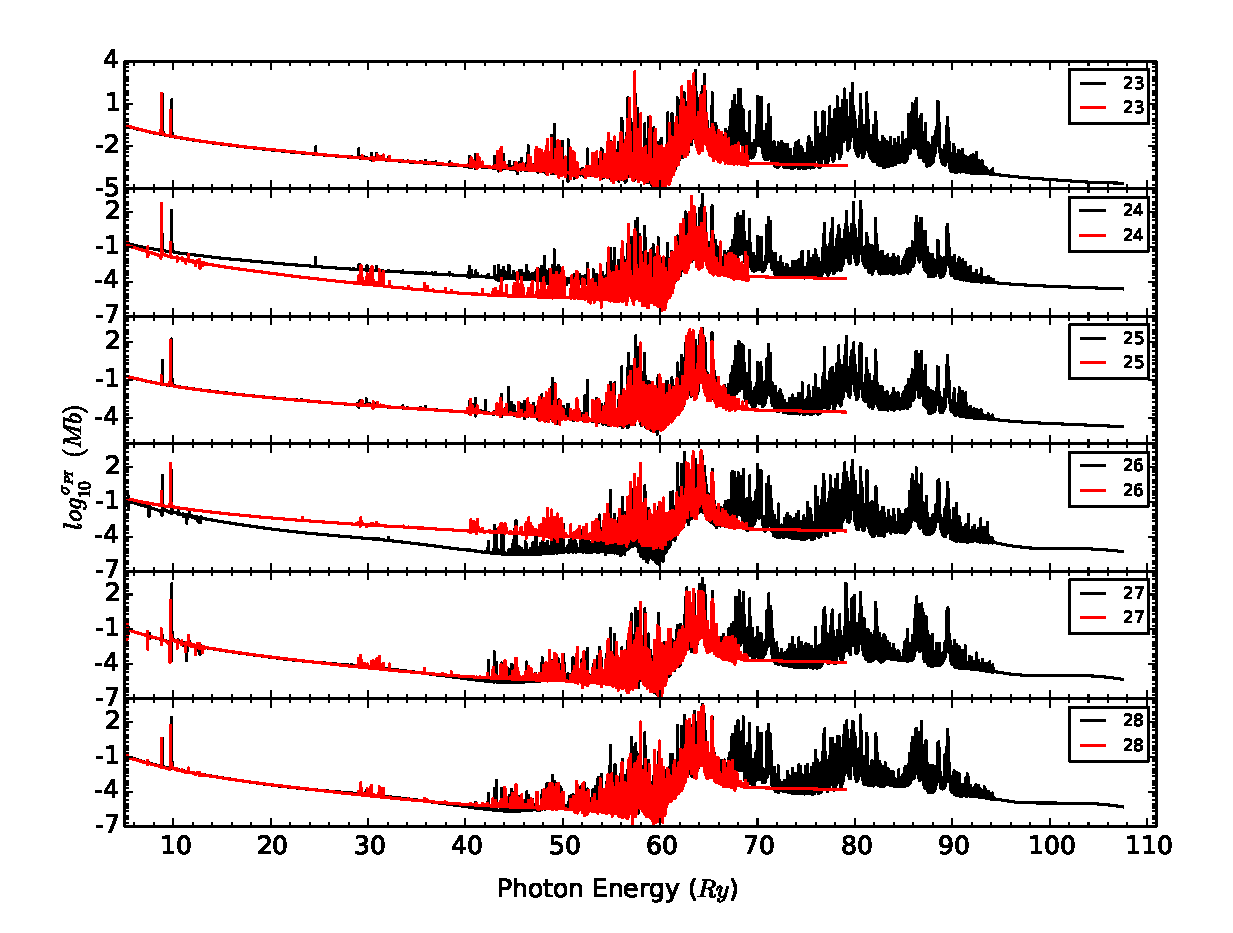
\includegraphics[width=0.49\textwidth]{figures/fe17_n3_n4_mismatch}
		\label{fe17_n3_n4_mismatch}
	}
~
	\subfloat[\ion{Fe}{xviii}: before level 31 and 33 being switched]{
		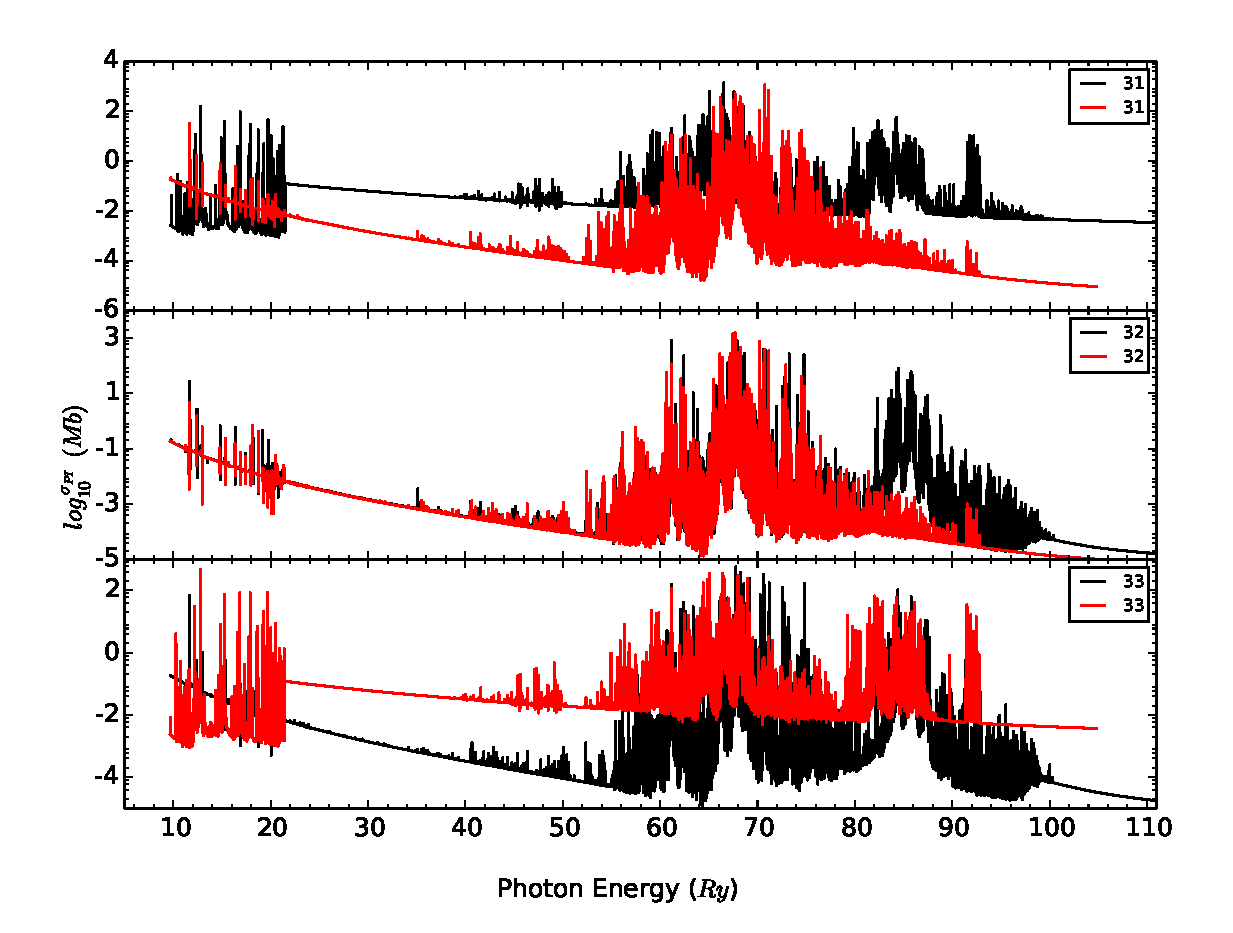
\includegraphics[width=0.49\textwidth]{figures/fe18_n3_n4_mismatch}
		\label{fe18_n3_n4_mismatch}
	}
	
	\subfloat[\ion{Fe}{xvii}: after level 24 and 26 being switched]{
		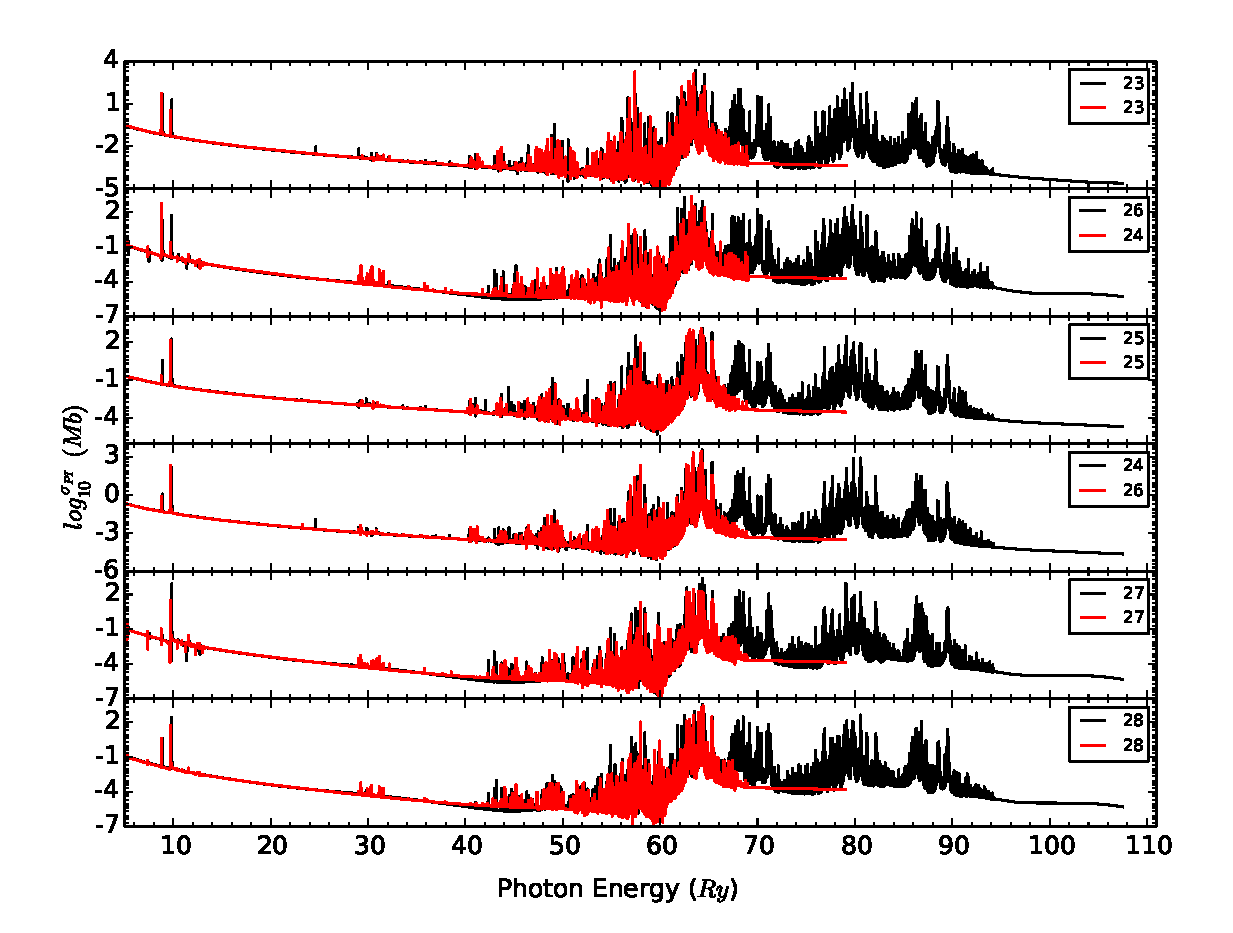
\includegraphics[width=0.49\textwidth]{figures/fe17_n3_n4_rematch}
		\label{fe17_n3_n4_rematch}
	}
~
	\subfloat[\ion{Fe}{xviii}: after level 31 and 33 being switched]{
		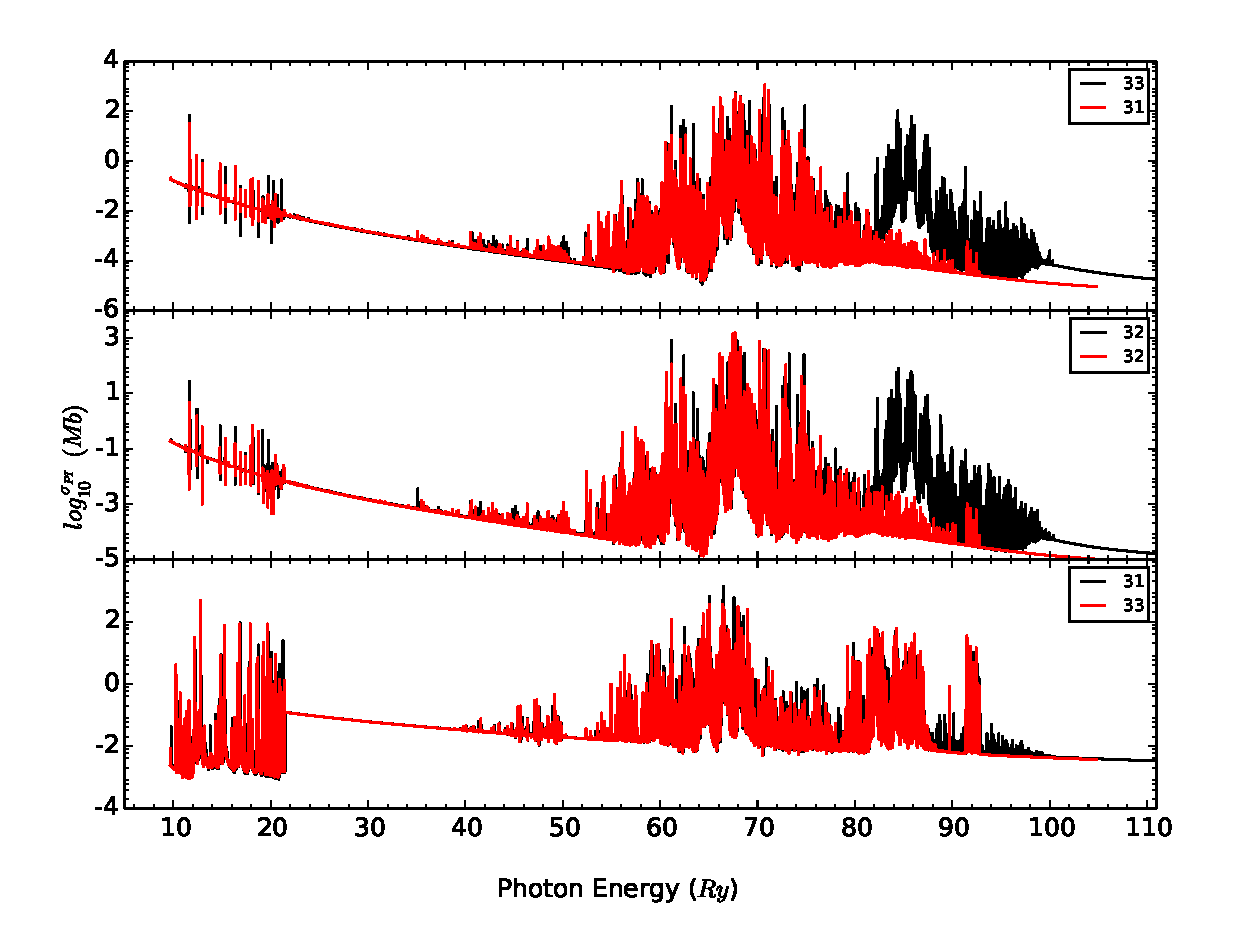
\includegraphics[width=0.49\textwidth]{figures/fe18_n3_n4_rematch}
		\label{fe18_n3_n4_rematch}
	}
	\caption{Photoionization cross section of 6 closely packed levels for \ion{Fe}{xvii} and 3 levels for \ion{Fe}{xviii} before and after being swtiched. \subref{fe17_n3_n4_mismatch}, \subref{fe18_n3_n4_mismatch}:  60CC-BPRM (red), 218CC-BPRM (black); \subref{fe17_n3_n4_rematch}, \subref{fe18_n3_n4_rematch}: 200CC-BPRM (red), 276CC-BPRM (black)}
	\label{mismatch}
\end{figure}

%=========== 3. TOPUP
\section{Top-Up}
Opacity project \citep{opcd_1, opcd_2} used close-coupling approximation and $R$-Matrix method to calculate photoionization cross section in the low energy region, and adopted a Kramer approximation fit afterwards \citep{opcd_7}. \citet{zhang_1998} replaced the Kramer tails with the relativistic distorted wave results including the contribution from inner-shell processes. Later opacity talbes were updated through including inner-shell transitions calculated by AUTOSTRUCTURE \citep{config_2003, config_2005}. In this section, we describe the procedure employed to match the bound state levels from BPRM and FAC calculations, and detail the bound-bound and bound-free top up calculation. Along the way, we discuss the effect of configuration interaction on the photoionization cross section. 

In diagram \ref{figure_topup_graph}, the black lines on the left indicate the core states that are already included in BPRM calculation, and the black lines on the right indicate the bound and quasi-bound levels that are considered in BPRM calculation. So the topup work is to include other core states up to principal quantum number $n=10$ (red lines on the left), and other pure bound levels (red lines indicated below $E=0$). For the bound levels that are already included in BPRM calculation, we first need to extend the calculation of direct photoionization to $500Ry$, then add the contribution due to the red lines on the left. For the unincluded bound levels, we need to calculation the direct photoionization due to all the core states. To simulate the autoionization resonances, we calculate the oscillator strength from the pure-bound levels to the red quasi-bound levels on the right. In addition we also include the bound-pure-bound transitions involving the unincluded bound levels (red lines below  $E=0$).
%======= FIGURE: topup_graph
\begin{figure}
	\centering
	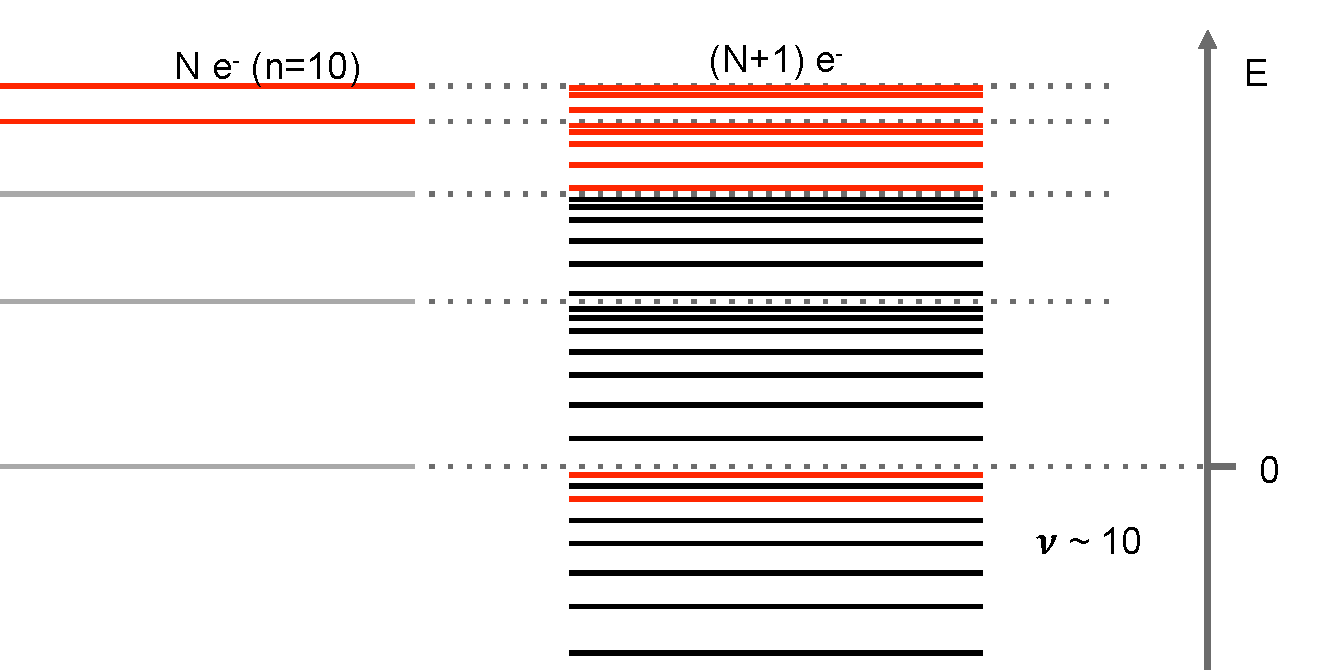
\includegraphics[width=.9\textwidth]{figures/topup_graph}	
	\caption{A diagram showing where the topup is done. Red: untreated in BPRM calculation; black: treated in BPRM calculation.}
	\label{figure_topup_graph}
\end{figure}

\subsection{Matching} \label{section_matching}
In BPRM calculation, the continuum orbitals $\ell\leq9$, the effective quantum number $\nu\leq10.1$, and the bound state levels can only be formed by coupling the $n=2$ core states with the continuum orbitals. So in FAC, we set the bound configurations as a permutation of the $n=2$ core configurations and an outer electron with principle quantumn number $n\leq10$. With only the same n-complex configuration interaction included, atomic structure is solved, sorted by total angular momentum $J$ and parity $\pi$, and ordered in energy, we find excellent agreement in the enregy between BPRM and FAC.

In calculating photoionization cross section, we include the whole n-complex of the core configurations for configuration interaction purpose, but only the transitions to the core configurations that are included in BPRM calculation are calculated. To delineate the edges of the photoionization cross section, the energy mesh is created in such a way that within any adjacent thresholds, 10 points are uniformly assigned. The partial photoionization cross section is computed in the default 6 energy grids, and interpolated/extrapolated in our mesh, and summed to give the toal photoionization cross section for each bound state level. To investigate the effect of configuration interaction on the photoionization cross section, two sets of RDW calculation are carried out. Both sets only allow the same-n-complex configuration interaction for bound configurations, but for the core configurations, one of them only allows the same-n-complex configuration interaction, and the other allows different-n-complex configuration interaction and we mix all the core configurations together. In RDW calculation, the photoionization strength is the dipole operator matrix $<\psi_i|\mathbb{D}|\psi_f>$ involving the electron in the bound state to the continuum, and all other electrons in the $|\psi_i>$ and $|\psi_f>$ must stay the same if only same-n-complex configuration inteaction is allowed, and can be different if different-n-complex configuration interaction is considered \citep{gu_email}.

To match the bound state levels from BPRM and RDW, it's necessary to compare the photoionization cross section to ensure the correctness of matching. We plot the photoionization cross section of BPRM and RDW in the order of energy for each $J$, $\pi$ symmetry pair, and a level is matched when the energy and the photoionization cross section agree reasonably well (here the background of the BPRM data and RDW are compared). Even though the different-n-complex configuration interaction for core configurations is used to maximally reproduce the background of BPRM calculation, we use the energy of the ground state of $n=2$ core when same-n-complex configuration interaction is applied as a reference to calculate the energy of the bound levels, as we found in this way RDW gives energies that are more close to BPRM's results. The photoionization cross section of the majority of the bound levels shows excellent consistancy at the first attempt (see figure \ref{fe17_bprm_fac} for \ion{Fe}{xvii} and figure \ref{fe18_bprm_fac} for \ion{Fe}{xviii}, where term notation ( $S$ and $L$) can not be determined from FAC output for all levels, so only configuration and total angular momentum $J$ are given). However, when several levels have almost the same energy (see table \ref{table_levles_matching}), distinctive difference may occur in the photoionization cross section and these levels need to be switched till good matching is achieved  (See figure \ref{fe17_howtomatch} for \ion{Fe}{xvii} and figure \ref{fe18_howtomatch} for \ion{Fe}{xviii}. Note: all the photoionization cross section of BPRM calculation includes a small region below the lowest ionization threshold for each level \citep{opcd_4}, where no RDW data is shown. ). In table \ref{table_levles_matching}, we can see the energy levels computed in BPRM and RDW agree quite well. For \ion{Fe}{xvii}, levels 13 and 14 , and levels 15 and 16 lie very close to each other, and in figure\ref{fe17_howtomatch}, levels 13 and 16 achieve good agreement, while levels 14 and 15 do not. So we switch the order of levels 14 and 15 in RDW calculation and recompare. Good agreement is achieved. Thus levels 13 - 16 in BPRM calculation are matched with those in RDW calculation. The same procedure is applied to levels 65 and 66 of \ion{Fe}{xviii} in table \ref{table_levles_matching}, and the result is shown in figure \ref{fe18_howtomatch}. When several levels are closely lying together and their BPRM photoionization cross section data are almost indistinguishable, exact matching in this way is lack of confidence, and the top up calculation performed on these levels may not correctly add the right tail to BPRM data (see section \ref{section_tail}), or add the contribution from the correct other-core configurations to the tailed BPRM data (see section \ref{section_other_targets}), but this will not make an impact in the opacity calculation as these levels have the same symmetry, almost the same energies, and almost the same photoionization cross section.

Usually it is rare to have more levels found in BPRM than that in RDW in the corresponding region, because BPRM does this by scanning the effective quantum number with a scanning step \citep{seaton_bound_1985, berrington_seaton_1985}, so it is possible that some of the levels that have very similar effective quantum number are missed out by such scanning technique, while RDW does an atomic structure calculation, i.e. including all the possible levels formed by electron quantum number coupling. However, such peculiar case happens in symmetry $J = 7/2, \pi = o$ of \ion{Fe}{xviii}. See table \ref{table_fake_level}. Around energy of $-3.5*z^2*10^{-2} Ry$, where $z=18$, BPRM finds 3 levels by scanning, while RDW gives only 2 levels. And we can see that levels 27 and 28 only differ by the last digit. Checking their photoionization cross section (see figure \ref{figure_fake_level}), we can hardly find any difference between levels 27 and 28. Thus we believe that one of levels 27 and 28 is spurious, and it may be caused by the numerical errors in BPRM. However, without deeper investigation, we still took it in the opacity calculation. Thus, in symmetry $J = 7/2, \pi = o$, from level 29 (we chose 29, but it is better 28)on, level $i$ in BPRM is matched with level $(i-1)$ in RDW. Therefore, from this point of view, level shifting is crucial and photoionization cross section comparison is necessary when doing the level matching. 

For both \ion{Fe}{xvii} and \ion{Fe}{xviii}, all bound levels are matched between BPRM and RDW, with excellect agreement. But in symmetry $J = 17/2, \pi = e$ of \ion{Fe}{xviii}, there is a big gap in the energy region where no dense resonances appear. The reason for this is that in BPRM calculation, only symmetries $J = 15/2, \pi = e$ and $J = 17/2, \pi = e$ of the free states are considered (no information about $J = 19/2, \pi = e$ in stg2), thus the photoionization cross section in BPRM is lower. For a complete view of the comparasion of the photoionization cross section (with the right oscillating end removed in BPRM data, see section \ref{section_tail}), go to \url{https://github.com/zhao1157/PhD-Atomic-Physics/tree/master/fe17_fe18_matched_levels}. 

%========= Table fake levels 7_1_27-28
\begin{table}
	\centering
	\caption{\ion{Fe}{xviii}: In symmetry $J = 7/2,~\pi = o$ of \ion{Fe}{xviii}, around energy $-3.5$, BPRM finds 3 levels, while RDW gives 2 levels. Note: the energy is $z$-scaled, and in unit of $10^{-2} Ry$.}
	\begin{tabular}{|c|c|}
		\hline
		\multicolumn{2}{|c|}{BPRM} \\
		\hline
		index & energy \\	
		\hline
		26 & -3.657952 \\
		27 & -3.523161 \\
		28 & -3.523163 \\
		29 & -3.522445 \\
		30 & -3.101211 \\	
		\hline	
	\end{tabular}
	\quad
	\begin{tabular}{|c|c|}
		\hline
		\multicolumn{2}{|c|}{RDW} \\
		\hline
		index & energy \\	
		\hline
		26 & -3.63053 \\
		27 & -3.53045 \\
		28 & -3.52958 \\
		29 & -3.11294 \\
		30 & -2.92945 \\	
		\hline	
	\end{tabular}
	\label{table_fake_level}
\end{table}

%======= FIGURE: 7_1_27-28 fake levels
\begin{figure}
	\centering
	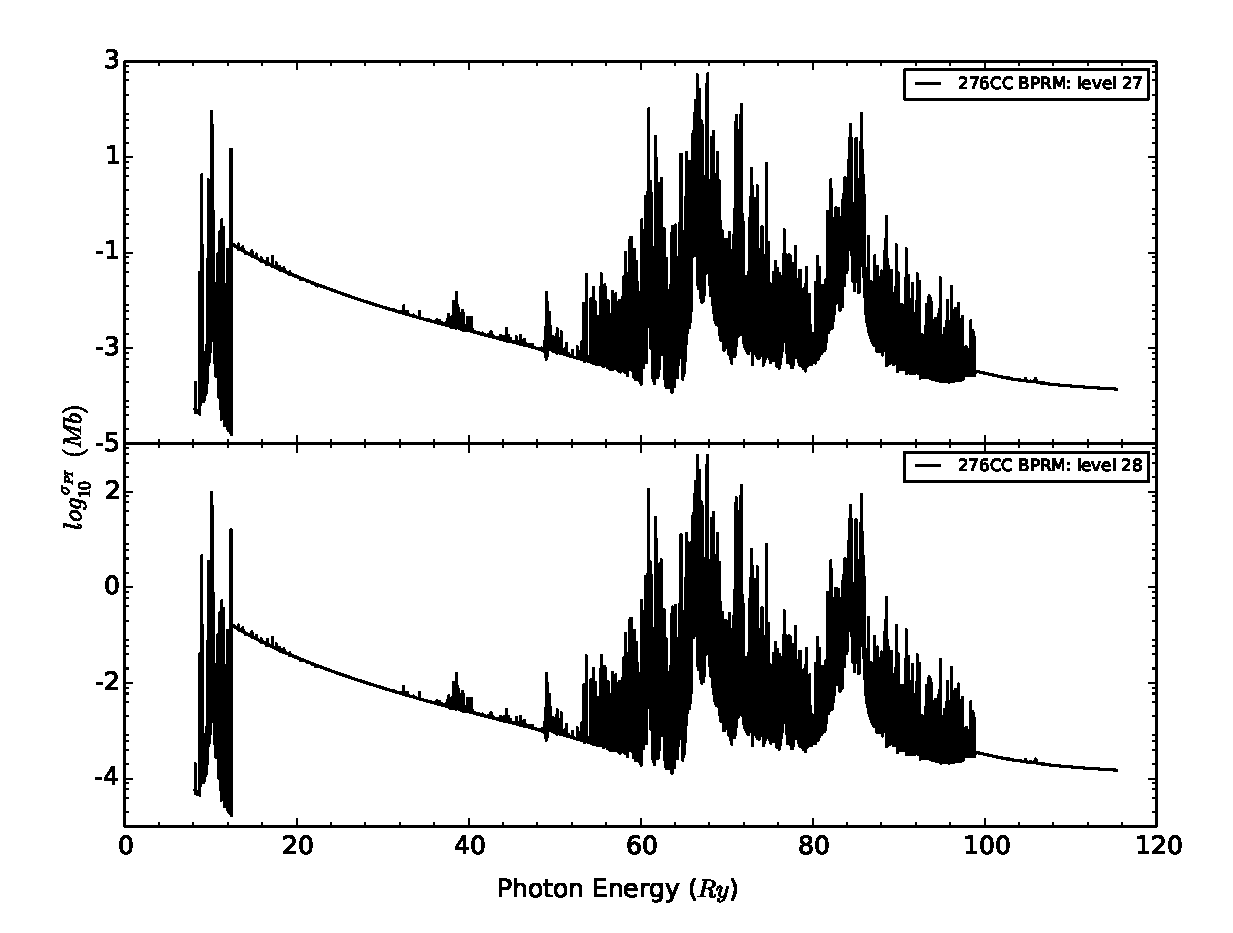
\includegraphics[width=.9\textwidth]{figures/fe18_fake_levels.eps}	
	\caption{\ion{Fe}{xviii}: The photoionization cross section of levels 27 and 28 as shown in table \ref{table_fake_level}.}
	\label{figure_fake_level}
\end{figure}




In figures \ref{fe17_bprm_fac}, \ref{fe18_bprm_fac}, \ref{fe17_howtomatch} \ref{fe18_howtomatch}, we show two sets of RDW calculation as described above and study the effect of configuration interaction on the photoionization cross section. Take the upper panel of figure \ref{fe17_bprm_fac} as an example. The configuration of the bound state after being matched with RDW is $2s^2 2p^5 4d$, so with only same-n-complex configuration interaction of the core configurations considered, the transitions can only happen to core configurations $2s^2 2p^5$, $2s 2p^5 4\ell$, $2s^2 2p^4 4\ell$ and $2p^6 4\ell$, where $\ell=s, p, d$, while with different-n-complex configuration interaction of the core configurations considered, additional contribution can be from all other core configurations. From  the upper panel of figure \ref{fe17_bprm_fac} we can see that same-n-complex configuratoin interaction gives pretty good background, though with some big gaps, while different-n-complex configuration interaction fills up such a big gap and improves the background significantly. The similar phenomenon can be found in the rest of the figures  \ref{fe17_bprm_fac}, \ref{fe18_bprm_fac}, \ref{fe17_howtomatch} \ref{fe18_howtomatch}, and there are still some gaps remaining after different-n-complex configuration interaction is allowed (Note: in figure \ref{fe18_bprm_fac} and \ref{fe18_howtomatch}, the oscillation in the background of the BPRM data can be eliminated with a larger number of continuum basis functions \citep{zhang_1998}).

Before deciding considering the different-n-complex configuration interaction of only the core configurations, we did the RDW calculation with different-n-complex configuration interaction of the bound configurations, i.e. putting all the bound configurations in just one $Structure()$ funciton in FAC. The result is not good when compared with BPRM result. Take levels 3 and 18 in symmetry $J=0,~\pi=e$ of \ion{Fe}{xvii} as an example. In figure \ref{figure_fe17_bound_mix}, we can see that with only same-n-complex configuration interaction of the bound configurations, RDW gives great result, while different-n-complex configuration interaction of the bound configurations makes the lower energy transitions worse. Thus in the level-matching process, to be consistent with BPRM result, we only consider the same-n-complex configuration interaction for the bound configurations, and different-n-complex configuration interaction for the core configurations. So is it in the top up calculation. 


%======== TABLE: closely packed levels in matching ======
\begin{table}
	\centering
	\caption {Selected levels of \ion{Fe}{xvii} ($J = 3, \pi = e$) and \ion{Fe}{xviii} ($J=1/2, \pi=e$) to be matched (Note: the energy is $z$-scaled, and in unit of $10^{-2} Ry$)}
	\begin{tabular}{|c || c | c | c|}
		\hline
		& level index & BPRM & RDW \\
		\hline
		\multirow{6}{*}{\ion{Fe}{xvii}} & 12 & -3.670657 & -3.67960 \\
		& 13 & -2.873930 & -2.84319 \\
		& 14 & -2.868775 & -2.84238 \\
		& 15 & -2.842915 & -2.83761 \\
		& 16 & -2.835625 & -2.83555 \\
		& 17 & -2.774853 & -2.77998 \\
		\hline
		\hline
		& level index & BPRM & RDW \\
		\hline
		\multirow{4}{*}{\ion{Fe}{xviii}} & 64 & -1.275887 & -1.27703  \\
		& 65 & -1.234865 & -1.24175 \\
		& 66 & -1.226084 & -1.23724 \\
		& 67 & -1.136909 & -1.14691 \\
		\hline
	\end{tabular}	
	\label{table_levles_matching}
\end{table}



%======= FIGURE: bprm and fac match
\begin{figure}
	\centering
		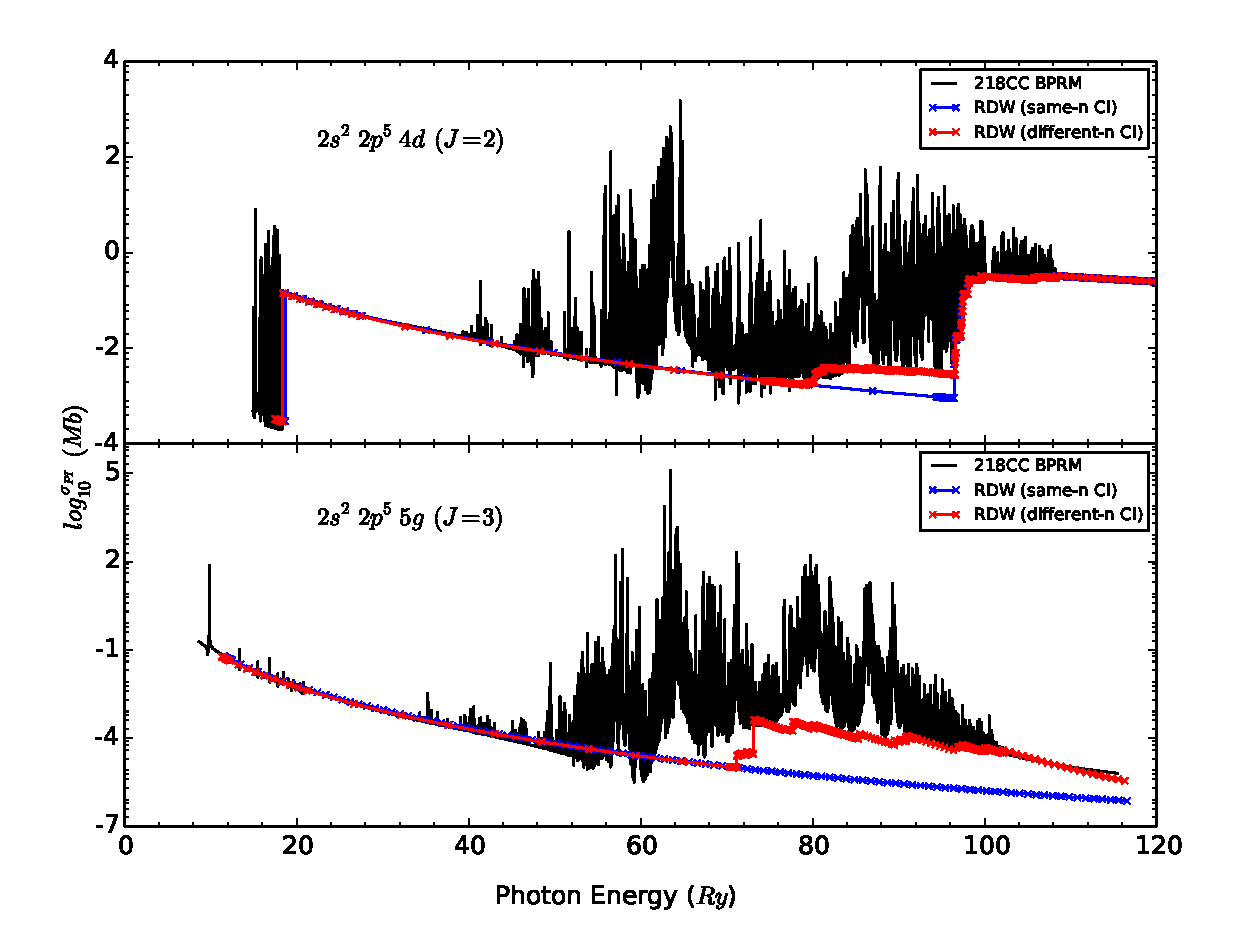
\includegraphics[width=.9\textwidth]{figures/fe17_bprm_fac.eps}	
	\caption{\ion{Fe}{xvii}: Most of the levels are matched at the first attempt with excellent consistency in photoionization cross section. The configuration is attached with each levle. BPRM (black), RDW(blue and red). ``Same-n CI'' means only same-n-complex configuration interaction is considered for core configurations, and ``different-n CI'' refers to both same-n- and different-n-complex configuration interaction is considered.}
	\label{fe17_bprm_fac}
\end{figure}

\begin{figure}
	\centering
	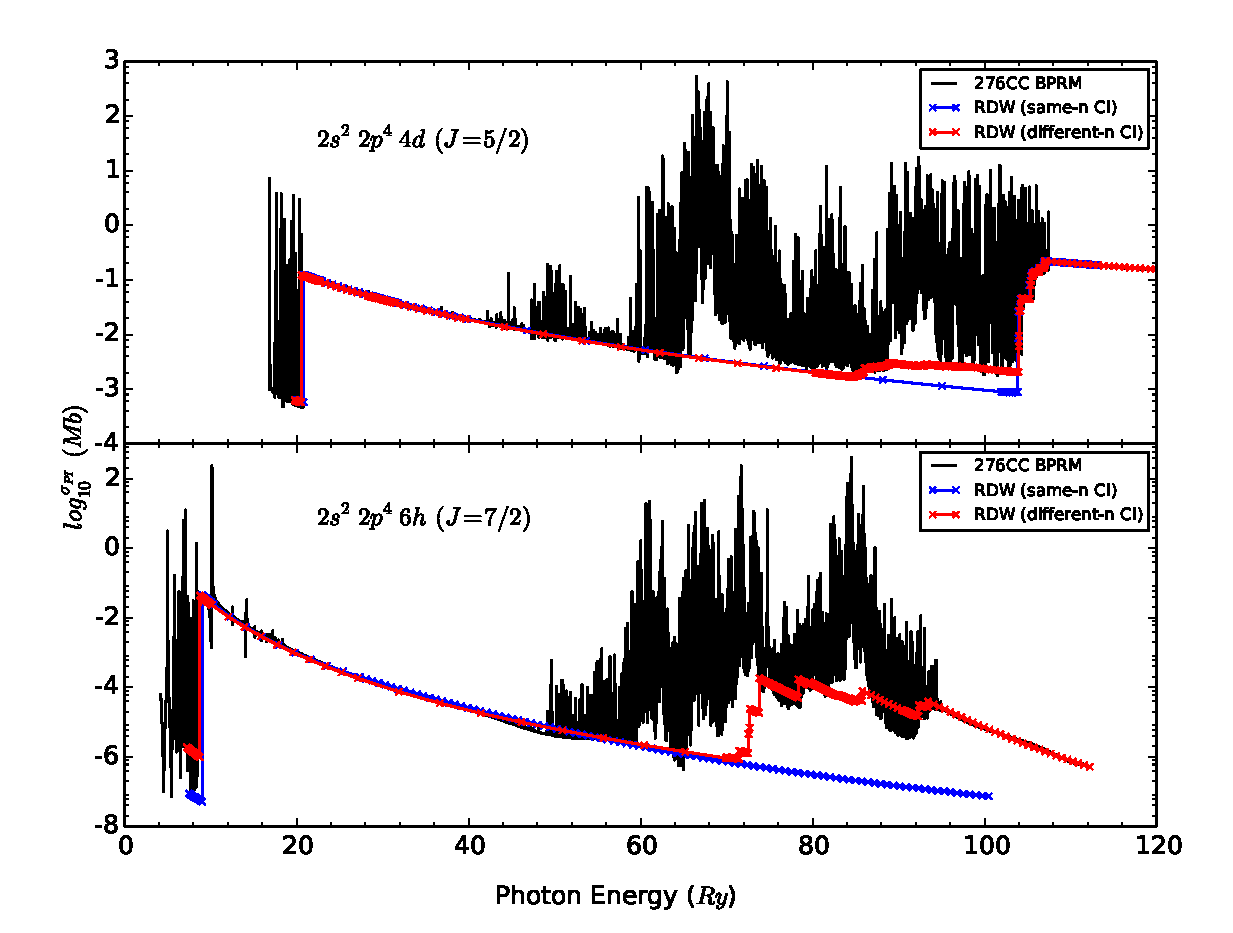
\includegraphics[width=.9\textwidth]{figures/fe18_bprm_fac.eps}
	\caption{\ion{Fe}{xviii}: Most of the levels are matched at the first attempt with excellent consistency in photoionization cross section. The configuration is attached with each levle. BPRM (black), RDW(blue and red). ``Same-n CI'' means only same-n-complex configuration interaction is considered for core configurations, and ``different-n CI'' refers to both same-n- and different-n-complex configuration interaction is considered.}
	\label{fe18_bprm_fac}
\end{figure}

%=========Figure: HOWTOMATCH
\begin{figure}
	\centering
	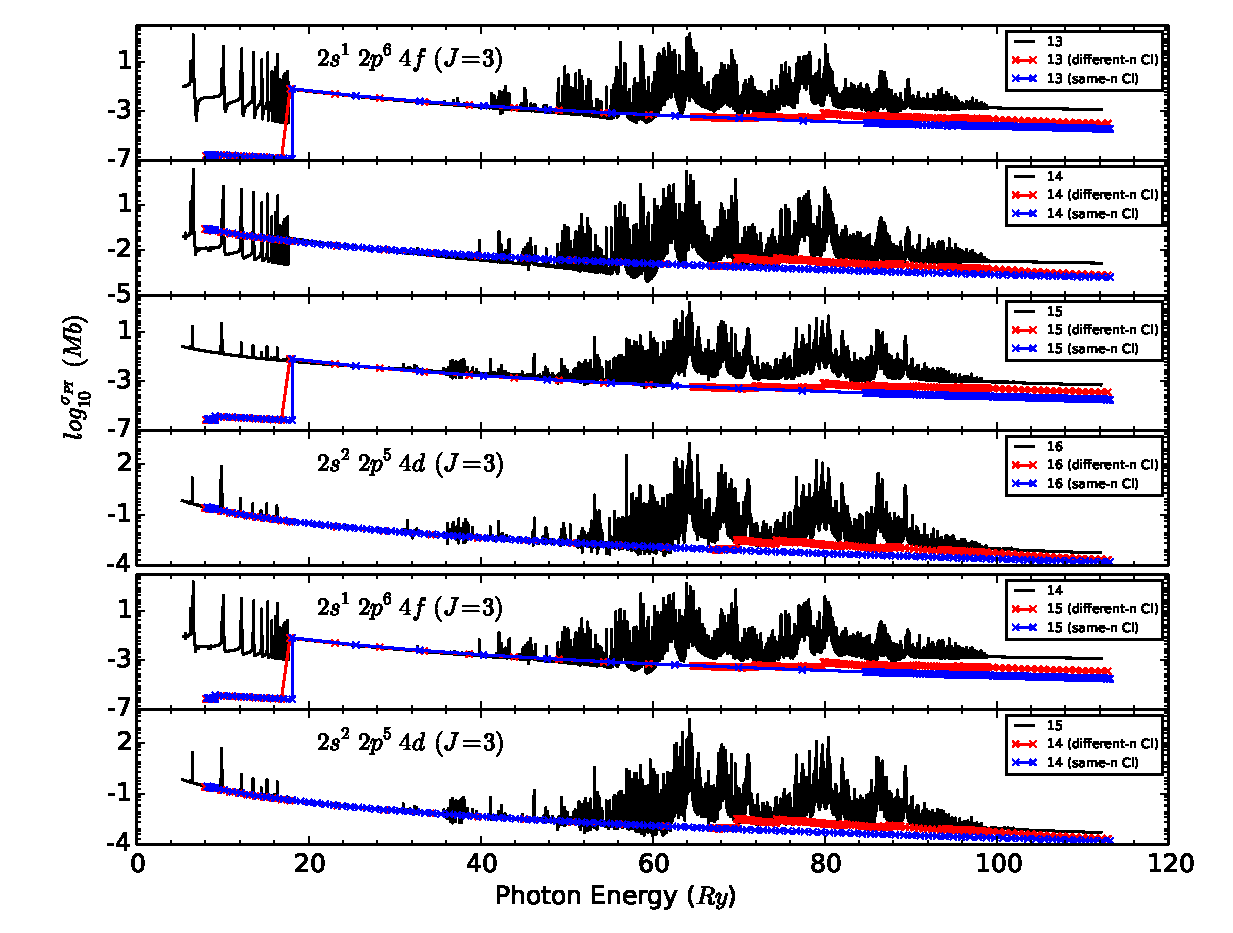
\includegraphics[width=.9\textwidth]{figures/fe17_howtomatch.eps}
	\caption{\ion{Fe}{xvii}: Multiple attemps are needed to ensure the correct matching when the levels are found with discrepancy in the photoionization cross section. The discrepancy is shown in upper panel and the final matching is in the lower one. Find the confuration attached for each level. BPRM (black), RDW(blue and red). ``Same-n CI'' refers to only same-n-complex configuration interaction is considered for core configurations, and ``different-n CI'' refers to both same-n- and different-n-complex configuration interaction are considered.}
	\label{fe17_howtomatch}
\end{figure}

\begin{figure}
	\centering
		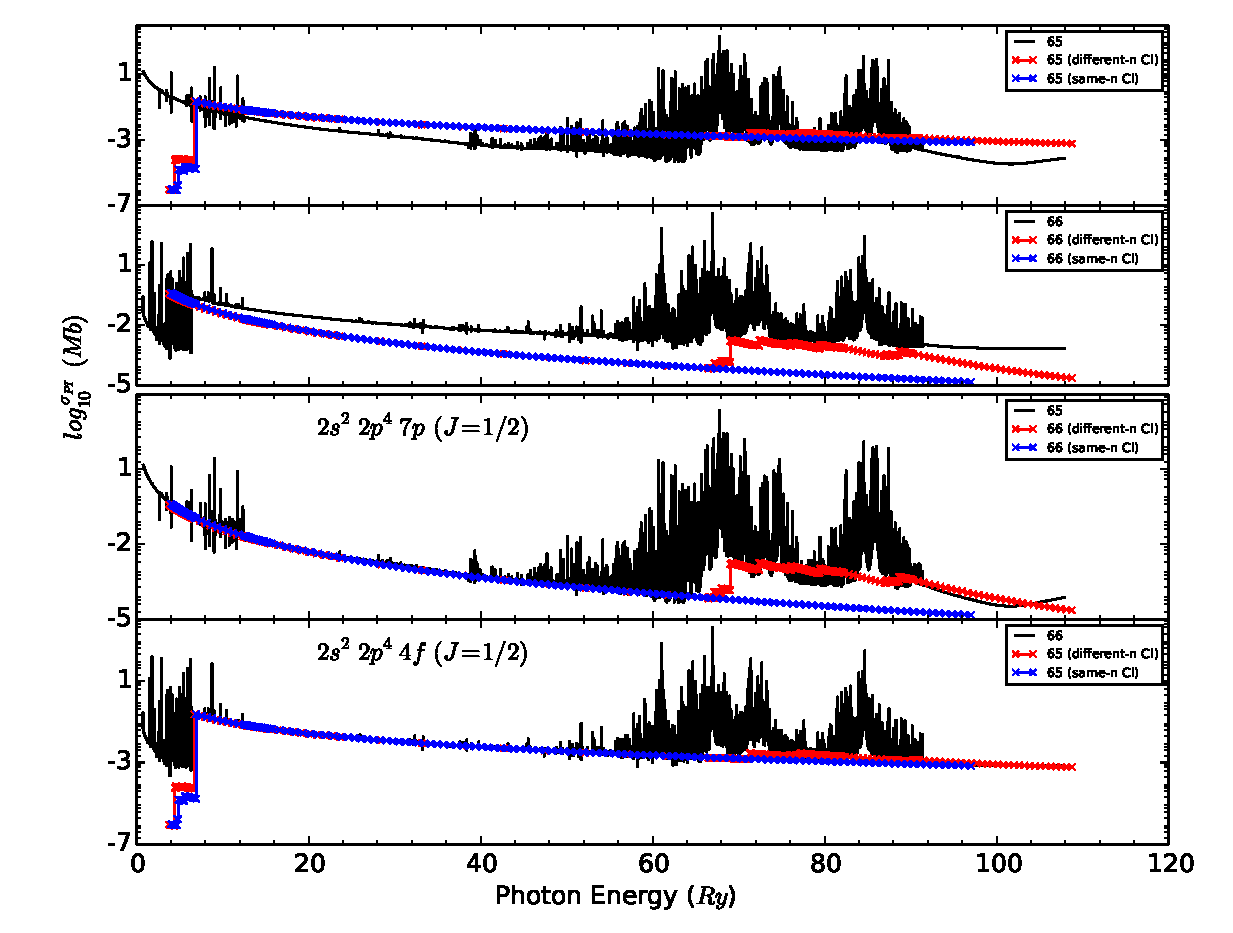
\includegraphics[width=.9\textwidth]{figures/fe18_howtomatch.eps}
	\caption{\ion{Fe}{xviii}: Multiple attemps are needed to ensure the correct matching when the levels are found with discrepancy in the photoionization cross section.The discrepancy is shown in upper panel and the final matching is in the lower one. Find the confuration attached for each level. BPRM (black), RDW(blue and red). ``Same-n CI'' refers to only same-n-complex configuration interaction is considered for core configurations, and ``different-n CI'' refers to both same-n- and different-n-complex configuration interaction are considered.}
	\label{fe18_howtomatch}
\end{figure}

%=========Figure: bound configurations mix
\begin{figure}
	\centering
	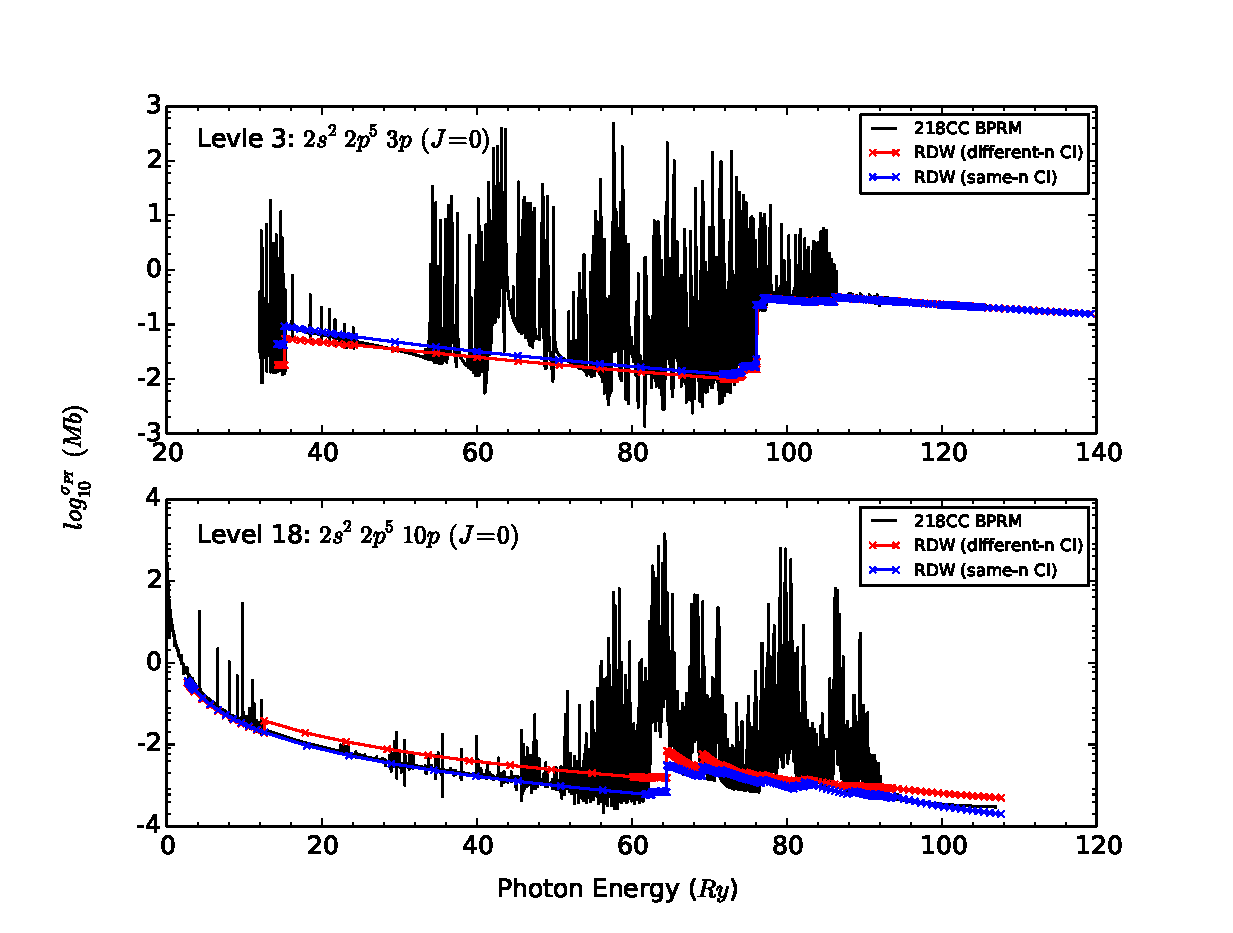
\includegraphics[width=.9\textwidth]{figures/fe17_bound_mix.eps}
	\caption{\ion{Fe}{xvii} ($J = 0, ~\pi=e$): BPRM (black), RDW(blue and red). In addition to the different-n-complex configuration interaction of the core configurations included, the configuration interaction of the bound configurations is tested.  ``Same-n CI'' refers to only same-n-complex configuration interaction is considered for the bound configurations, and ``different-n CI'' refers to both same-n- and different-n-complex configuration interaction are considered.}
	\label{figure_fe17_bound_mix}
\end{figure}


\subsection{Bound - Free} \label{section_bf}
As BPRM calculation is carried out in the lower part of the whole energy range, and it inlucdes low-n core configurations, we use RDW to extend it to higher region up to 500 $Ry$ of photoelectron energy, and to include high-n core configurations up tp $n=10$. The following part of the section gives detailed description of these aspects.

\subsubsection{Tail} \label{section_tail}
As shown in figures \ref{fe17_bprm_fac} and \ref{fe18_bprm_fac}, the RDW data can be matched almost perfectly to the background of BPRM result, however, we also find there are cases where they do not match well in the right region of energy. For example, in the top panels of figures \ref{fig_fe17_discrepancy} and \ref{fig_fe18_discrepancy}, different-n-complex CI introduces many transitions, but they are not strong enough to raise to the  background of BPRM. In the middle panel of figure \ref{fig_fe17_discrepancy}, different-n-complex CI introduces many edges at positions where the background of BPRM jumps, and raises the background higher than BPRM. While in the middle panel of figure \ref{fig_fe18_discrepancy}, around $105~Ry$, compared with same-n-complex CI, different-n-complex CI moves the background up on the left side, and down on the right side, i.e. converging to the background of BPRM.

Initially as only the same-n-complex CI was considered, there were big gaps between the background of BPRM and RDW for majority of the bound levels, and to extend the data to higher energy region, we multiplied the RDW data for each level by a ratio obtained at the last point of BPRM so that the values of BPRM and RDW are equal at that energy. When different-n-complex configuration interaction is considered, such big gaps are mostly filled up, though with some discrepancy for some levels, the same ``scaled-RDW'' tail treatment is applied and the distribution of the ratios are shown in figure \ref{fig_ratio} for both \ion{Fe}{xvii} and \ion{Fe}{xviii}. We can see that the distribution is very alike for both ions, and there are around $60\%$ of the bound levels lying around ratio of 1, and the rest are in high ratios. After further investigation, we find the high ratios are mainly caused by the oscillation of BPRM background, which is due to the small number of continuum basis funcitons used in the wavefunction expansion \citep{zhang_1998}. Please see the bottom panels of figures \ref{fig_fe17_discrepancy} and \ref{fig_fe18_discrepancy}. With such oscillation removed at the end of BPRM data (about the last 1000 points for each level), the ratios improve dramatically (see figure \ref{fig_ratio_no_oscillation}), and there are about $85\%$ of the levels are around ratio of 1. Through this distribution, we can have a glimpse of how well the levels are matched and how well the BPRM and RDW calculation agree with each other. But with further consideration, we set all the ratios to 1, i.e. take RDW data as it is, and add RDW tail directly to BPRM data just like what \citet{zhang_1998} did, because RDW is more accurate in the higher energy region and multiplying a ratio to RDW data introduces an obvious inaccuracy in that region, though without multiplying the ratio it causes a discontinuity in the data.

The energy mesh used in the region is created in such a way that 10 points are uniformly assigned beween any adjacent ionization thresholds due to the other core configurations (see section \ref{section_other_targets}).

%=========Figure: MATCH_DISCREPANCY
\begin{figure}
	\centering
	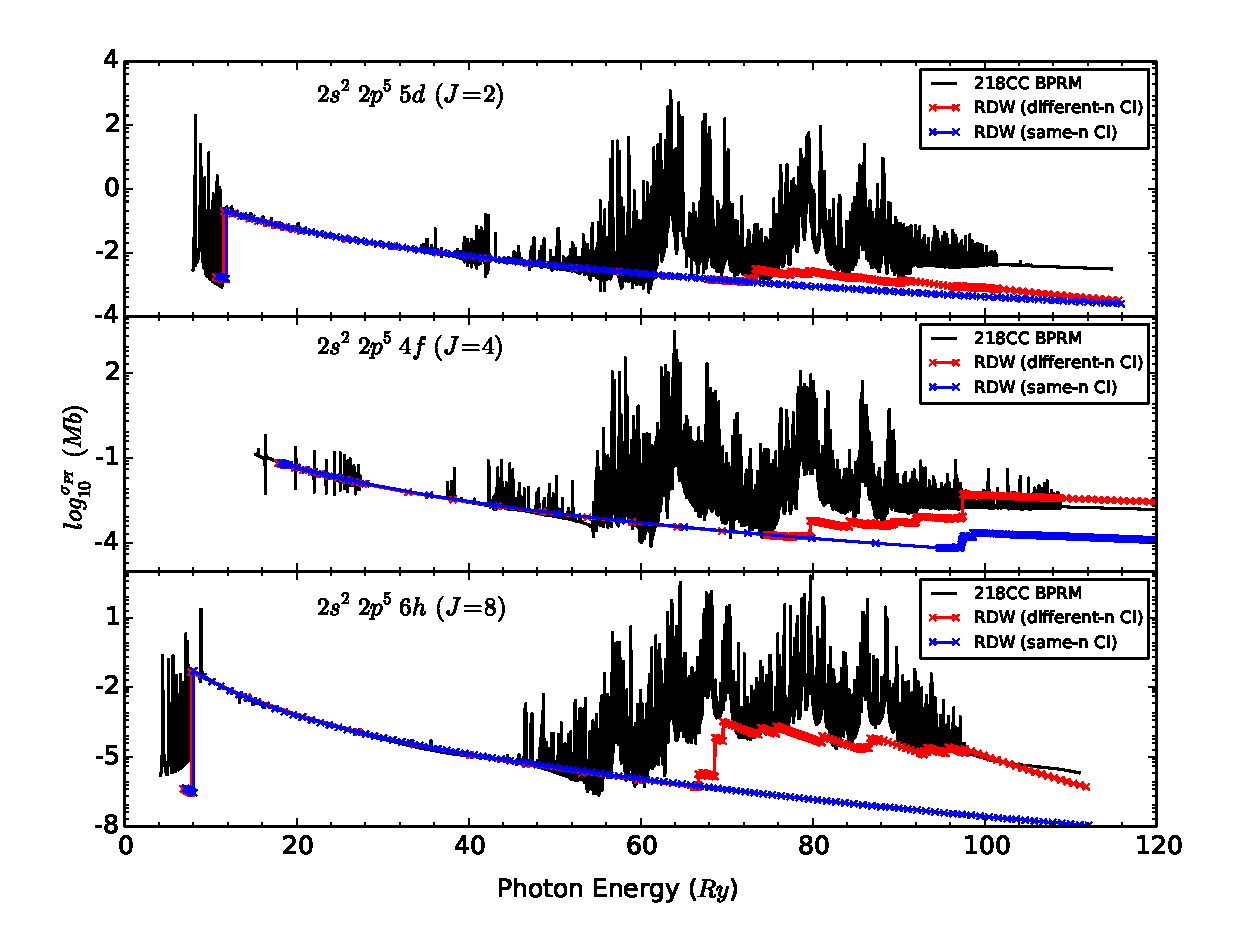
\includegraphics[width=.9\textwidth]{figures/fe17_discrepancy.eps}
	\caption{\ion{Fe}{xvii}: Different-n configuration interaction improves the background significantly, but there is still very large discrepancy in the right region of energy for some levels. BPRM (black), RDW(blue and red). ``Same-n CI'' refers to only same-n-complex configuration interaction is considered for core configurations, and ``different-n CI'' refers to both same-n- and different-n-complex configuration interaction are considered.}
	\label{fig_fe17_discrepancy}
\end{figure}

\begin{figure}
	\centering
	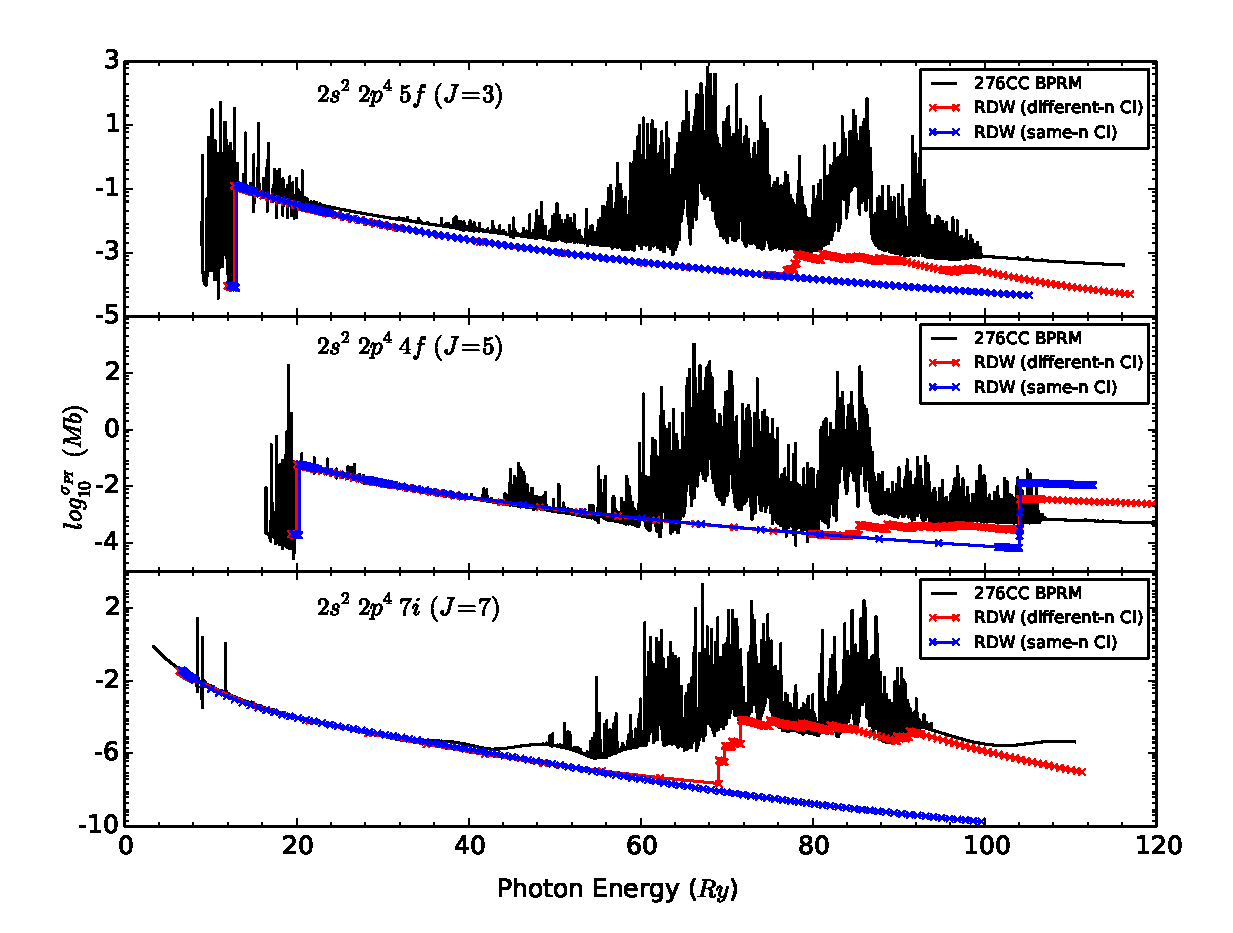
\includegraphics[width=.9\textwidth]{figures/fe18_discrepancy.eps}
	\caption{\ion{Fe}{xviii}: Different-n configuration interaction improves the background significantly, but there is still very large discrepancy in the right region of energy for some levels. BPRM (black), RDW(blue and red). ``Same-n CI'' refers to only same-n-complex configuration interaction is considered for core configurations, and ``different-n CI'' refers to both same-n- and different-n-complex configuration interaction are considered.}
	\label{fig_fe18_discrepancy}
\end{figure}

%=========Figure: RATIO with oscillation
\begin{figure}
	\centering
	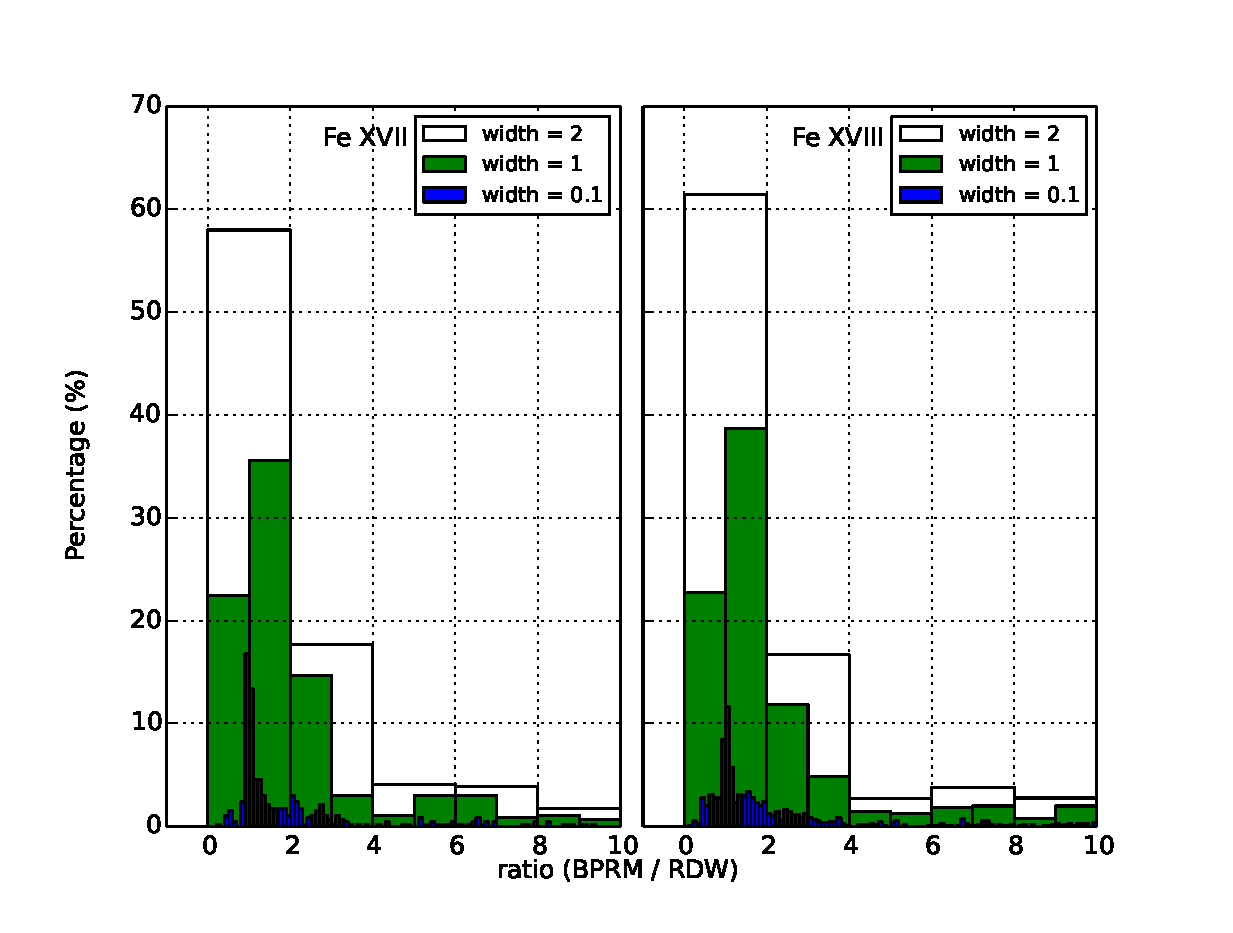
\includegraphics[width=0.9\textwidth]{figures/ratio_bprm_fac.eps}
	\caption{The distribution of the factors multiplied to RDW data in the higher energy region for \ion{Fe}{xvii} and \ion{Fe}{xviii} with the oscillating end of BPRM data included. ``width'' is the width of the bins. }
	\label{fig_ratio}
\end{figure}

%=========Figure: RATIO with NO oscillation
\begin{figure}
	\centering
	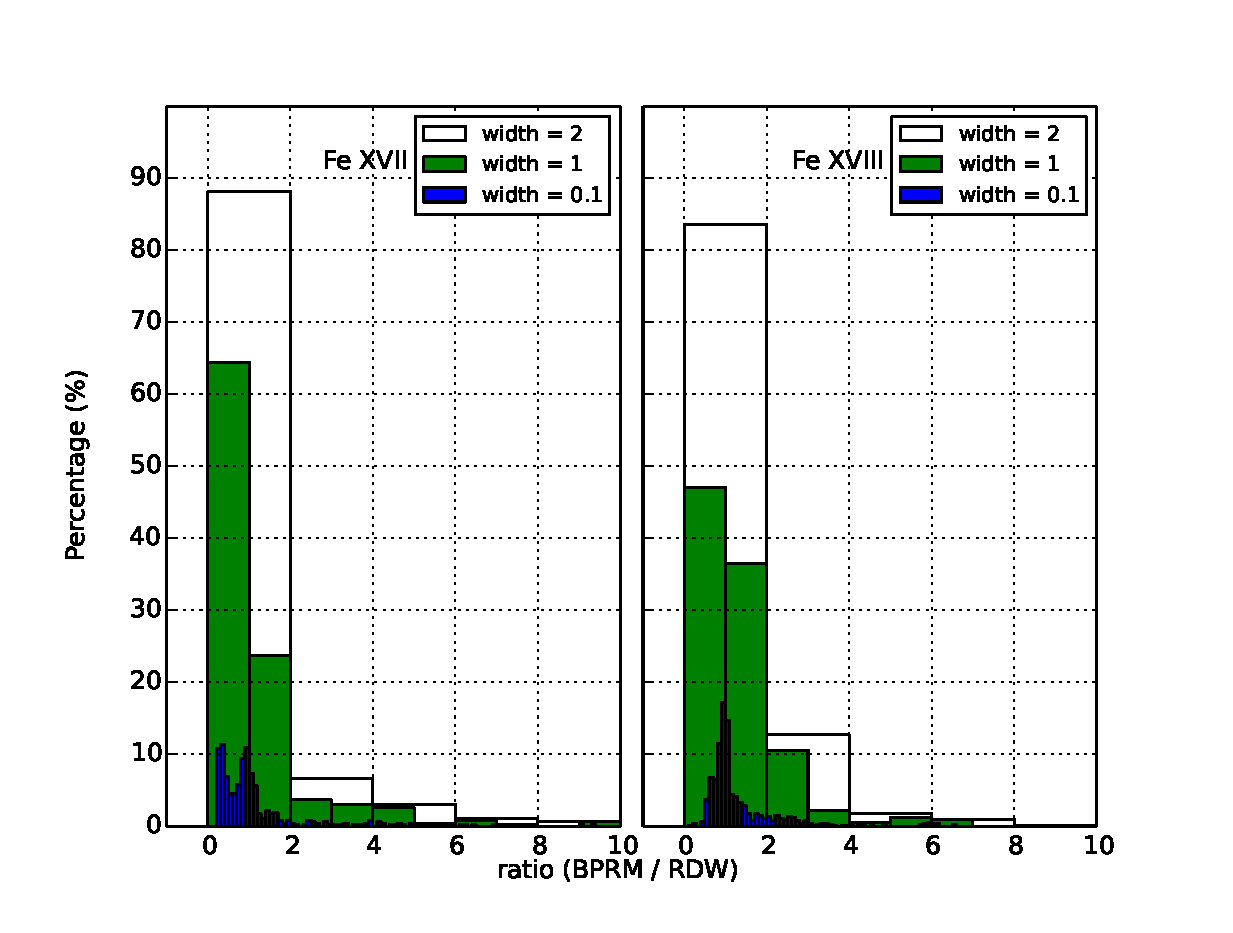
\includegraphics[width=0.9\textwidth]{figures/ratio_bprm_fac_no_oscillation.eps}
	\caption{The distribution of the factors multiplied to RDW data in the higher energy region for \ion{Fe}{xvii} and \ion{Fe}{xviii} \textbf{without} the oscillating end of BPRM data included. ``width'' is the width of the bins. }
	\label{fig_ratio_no_oscillation}
\end{figure}

\subsubsection{Other Core Configurations} \label{section_other_targets}
Using RDW with different-n-complex configuration interaction, we calculate photoionization cross section due to other core configurations up to $n=10$ that are not included in the BPRM calculation. As demonstrated in chapter \ref{chap_pec_l_edge}, the high-n core configurations are used to enable the convergence (jump) of the photoionization cross section of the high-n bound states. To top up 218CC BPRM for \ion{Fe}{xvii}, we include core configurations $2s^2 2p^4 4f$, $2s 2p^5 4f$, $2p^6 4\ell'$, and $2s^S 2p^P n\ell''$, where  $S$, $P$ are any possible non-negative integers satisfying $S+P=6$, $5 \leq n \leq 10$, and $\ell'$ and $\ell''$ are all possible subshells in the corresponding shell. To top up 276CC BPRM for \ion{Fe}{xviii}, we include core configurations $2p^5 3\ell$, $2s^2 2p^3 4f$, $2s 2p^4 4\ell'$,  $2p^5 4\ell''$,  $2s^S 2p^P n\ell'''$, where  $S$, $P$ are any possible non-negative integers satisfying $S+P=5$, $5 \leq n \leq 10$, and $\ell$, $\ell'$, $\ell''$ and $\ell'''$ are all possible subshells in the corresponding shell. The energy mesh is the same as the one used in BPRM calculation merged with the one in the high energy region as described in section \ref{section_tail}. 

As shown in figures \ref{fig_fe17_tail_other} and \ref{fig_fe18_tail_other}, the BPRM data is merged with the scaled RDW tail, and the contribution from other core configurations varies from negligible to noticeable. In table \ref{table_transition_other_core}, part of the transitions to the other core configurations are shown, which contribute most of the photoionizatoin cross section. Level $ 2s^2 2p^5 4d~(J=2) $ gets negligible contribution from the other core configurations compared with the tail, and the main transitions are due to different-n-complex configuration interaction. Levels $2s^2 2p^5 5g~(J=3)$, $2s^2 2p^4 4d~(J=5/2)$ and $2s^2 2p^4 6h~(J=7/2)$ have a good amount of contribution from the other core configurations, and they are mainly due to the same-n-complex configuration interaction, i.e. ionizing one electron from $L-$shell while keeping the other electrons unchanged. For level $2s^2 2p^4 4d~(J=5/2)$, since in 276 CCBPRM, core configuration $2s^2 2p^3 4d$ has been considered, leaving out $2s 2p^4 4d$, that is why only $2s 2p^4 4d$ contribute mainly in the top up calculation, and it is comparable with the BPRM tail, which is mainly due to the transitions to $2s^2 2p^3 4d$ (see table \ref{table_n3_n4_jumps}). 

To illustrate the statement made in section \ref{section_matching} that non-exact matching for closely lying levels does not make an impact on the accuracy of the top up data in terms of opacity calculation. Take level $2s^2 2p^4 6h~(J=7/2)$ as an example, which is level 44 as shown in table \ref{table_7_1_44}, in which levels 42 - 45 have almost the same energy and are distinctively different from levels 41 and 46, and once again BPRM and RDW calculations show a great agreement.  Figure  \ref{fig_7_1_44_not_matter} shows the photoionization cross section of these four levels, and we notice that even though those four levels have almost the same energy and the photoionization cross section look quite similar, levels 42 and 43 are more similar to each other while levels 44 and 45 look more similar to each other. It turns out levels 42 and 43 are from the same configuration $2s^2 2p^4 6f$ and levels 44 and 45 are from configuration $2s^2 2p^4 6h$. Thus for levels that have the same symmetry and very similar energy, the levels from the same configuration have very similar photoionization cross section, and it is impossible to distinguish them using our matching method. When doing the topup calculation, it does not matter which tail or contribution from other cores is added to which level among these indistinguishable levels. As shown in figure \ref{fig_7_1_44_not_matter_tail_other}, we can see that tails of levels 42 and 43 are essentially the same with negligible difference, so are the levels 44 and 45. And the contribution from other cores is also essentially the same. Thus there is really no need to distinguish them and the top up data is correctly added to the BPRM data.



%======== Table transitoins due to other cores
\begin{table}
	\centering
	\caption{Listed are some of the other core configurations which contribute most of the photoionization cross section for the four levles shown in figures \ref{fig_fe17_tail_other} and \ref{fig_fe18_tail_other}.}
	\begin{tabular} {|c ||c | c |}
		\hline
		Ion & Bound levels & Final configurations \\
		\hline
		\multirow{5}{*}{\ion{Fe}{xvii}} & \multirow{3}{*}{$2s^2 2p^5 4d~(J = 2)$} & $2s^2 2p^4 5d/5f/6d$ \\
																	   &  & $2s 2p^5 5d$ \\
																	   &  & $2p^6 4d$ \\
		\cline{2-3}
		&\multirow{2}{*}{$2s^2 2p^5 5g~(J = 3)$}  & $2s^2 2p^4 5g$ \\
																	   && $2s 2p^5 5g$ \\
		\hline
		\multirow{3}{*}{\ion{Fe}{xviii}} & \multirow{1}{*}{$2s^2 2p^4 4d~(J = 5/2)$}  & $2s 2p^4 4d$ \\
		\cline{2-3}
		& \multirow{2}{*}{$2s^2 2p^4 6h~(J = 7/2)$}  & $2s^2 2p^3 6h$ \\
																		 & & $2s 2p^4 6h$ \\
		\hline			  								   
	\end{tabular}
	\label{table_transition_other_core}
\end{table}

%=========Figure: TAIL_OTHER_TARGETS
\begin{figure}
	\centering
		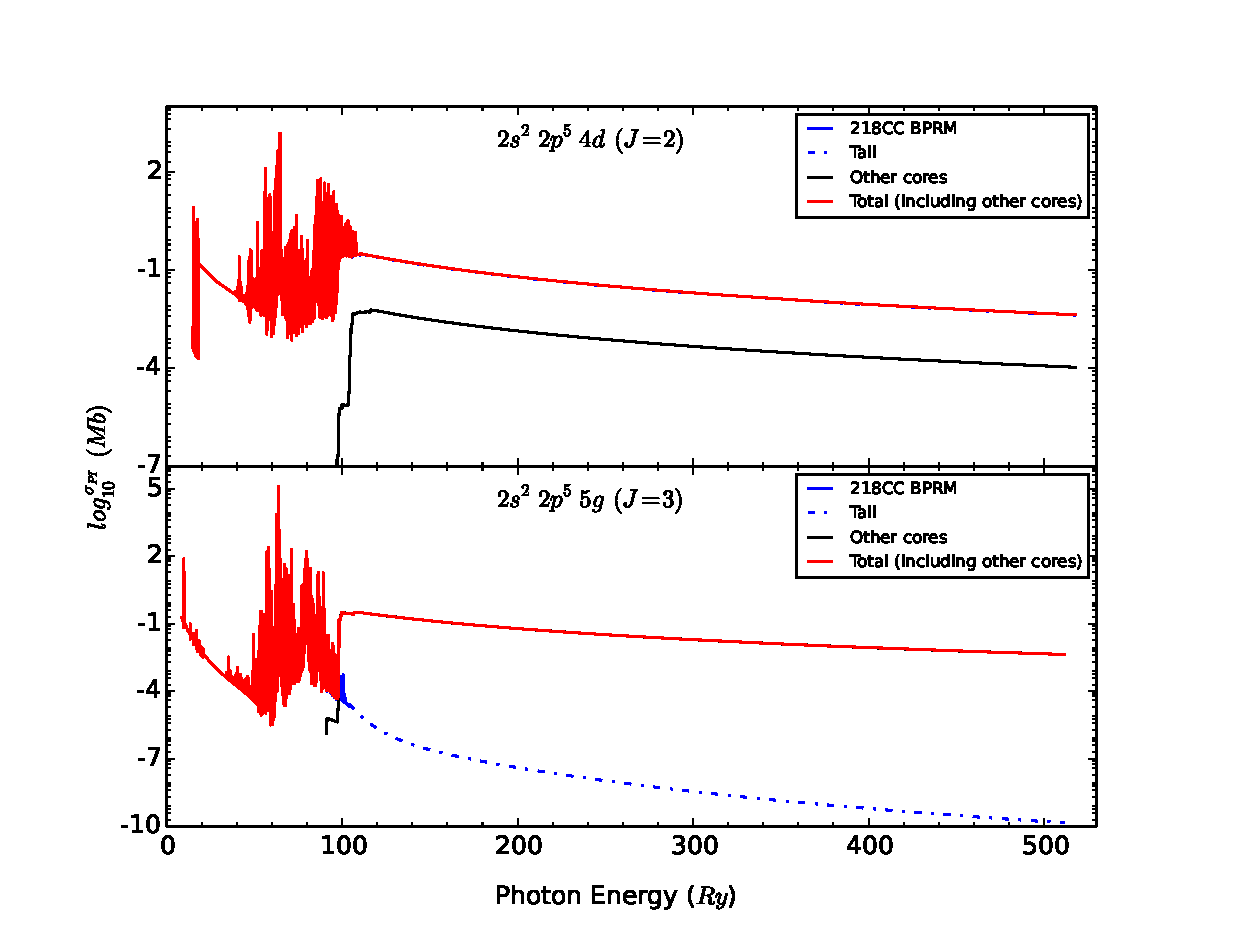
\includegraphics[width=.9\textwidth]{figures/fe17_tail_other_targets.eps}
	\caption{\ion{Fe}{xvii}: The photoinization cross section of the same four levels as in figure \ref{fe17_bprm_fac} are extended to higher enegy region and the contribution from other core configurations with different-n-complex configuration interaction is added. Blue (solid): BPRM calculation; blue (dash-dotted): RDW data; black: contribution from other core configurations; red: total photionization cross section.}
	\label{fig_fe17_tail_other}
\end{figure}

\begin{figure}
	\centering
		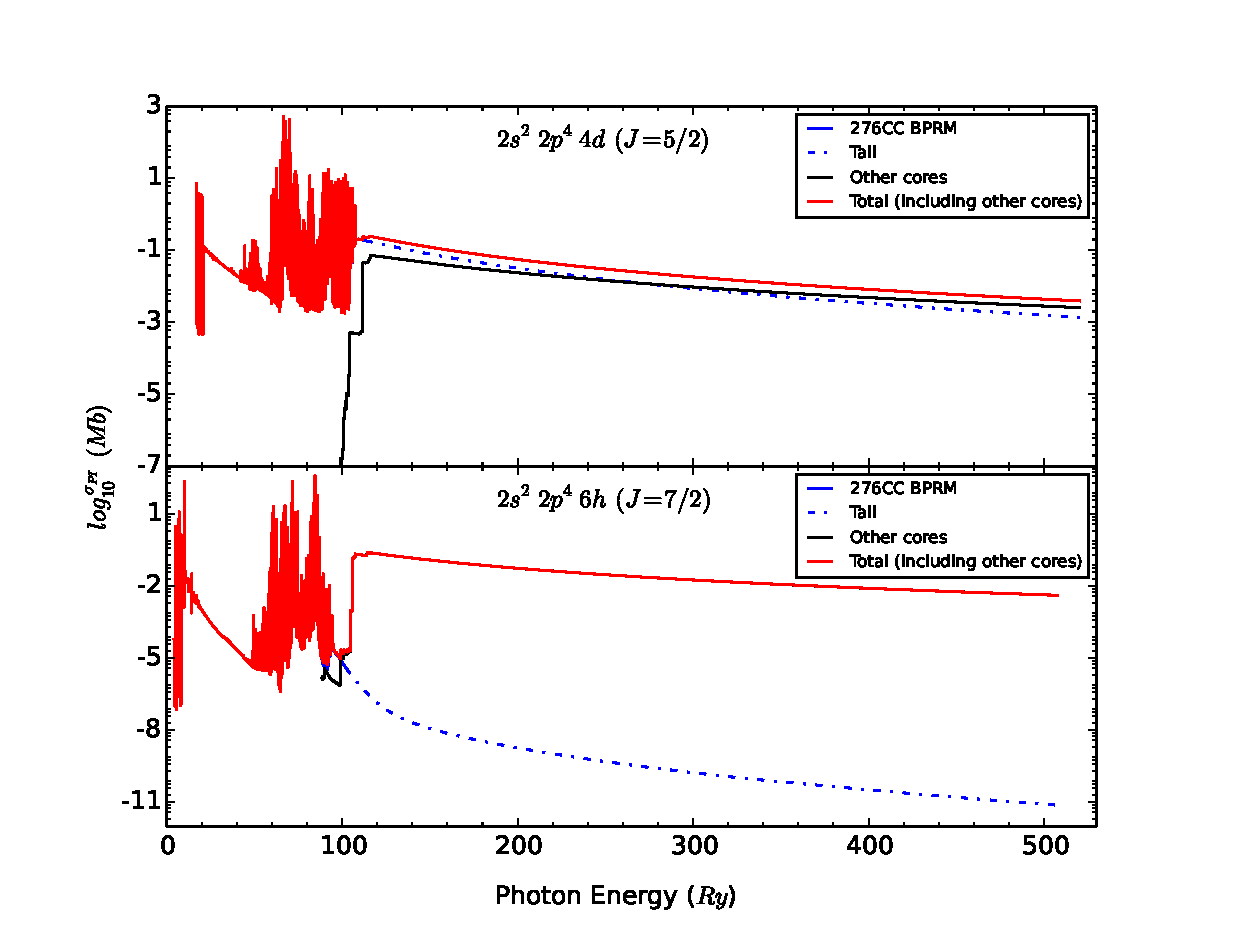
\includegraphics[width=.9\textwidth]{figures/fe18_tail_other_targets.eps}
	\caption{\ion{Fe}{xviii}: The photoinization cross section of the same four levels as in figure \ref{fe18_bprm_fac} are extended to higher enegy region and the contribution from other core configurations with different-n-complex configuration interaction is added. Blue (solid): BPRM calculation; blue (dash-dotted): RDW data; black: contribution from other core configurations; red: total photionization cross section.}
	\label{fig_fe18_tail_other}
\end{figure}


%======== Table 7_1_44 and 3 other closely lying levels
\begin{table}
	\centering
	\caption{Listed are four closely lying levels 42 - 45 with the same symmetry ($J = 7/2,~\pi = o$) for \ion{Fe}{xvii}, among which level 44 is the one shown in the bottom panel of figure \ref{fig_fe18_tail_other}. Note: the energy is $z$-scaled ($z=17$ for \ion{Fe}{xvii}), and in unit of $10^{-2} Ry$.}
	\begin{tabular} { |c || c | c |}
		\hline
		level index & BPRM & RDW \\
		\hline
		41 & -2.445974 & -2.45745 \\
		42 & -2.299232 & -2.30863 \\
		43 & -2.298194 & -2.30822 \\
		44 & -2.295646 & -2.30750 \\
		45 & -2.294440 & -2.30630 \\
		46 & -2.135242 & -2.13520 \\
		\hline	  								   
	\end{tabular}
	\label{table_7_1_44}
\end{table}

%======= Figure mismatch_not_matter 
\begin{figure}
	\centering
	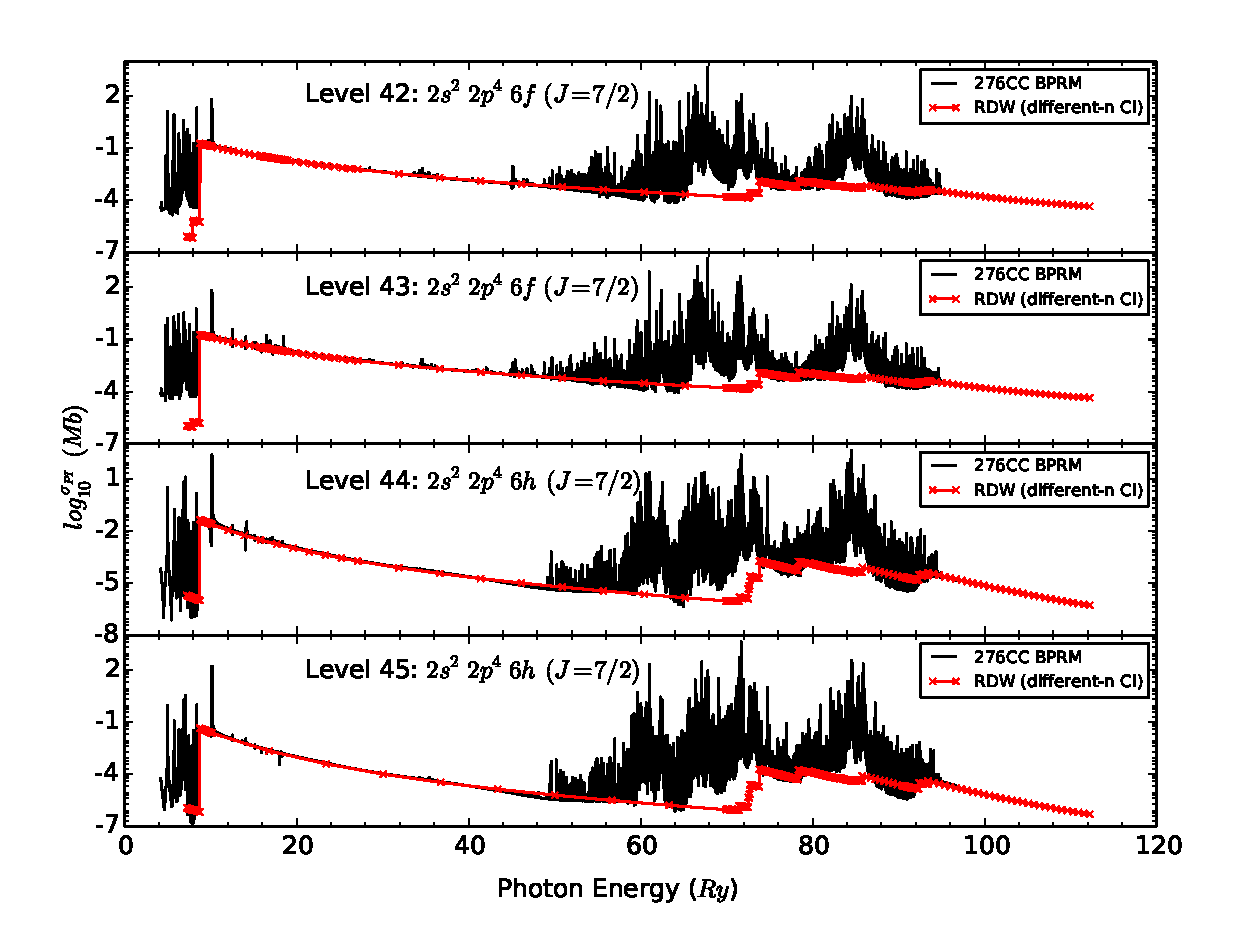
\includegraphics[width=\textwidth]{figures/fe18_mismatch_not_matter.eps}
	\caption{\ion{Fe}{xviii}: The photoionization cross section of levels 42 - 45 as shown in table \ref{table_7_1_44} for both BPRM and RDW. }
	\label{fig_7_1_44_not_matter}
\end{figure}

%======= Figure mismatch_not_matter_tail_other
\begin{figure}
	\centering
	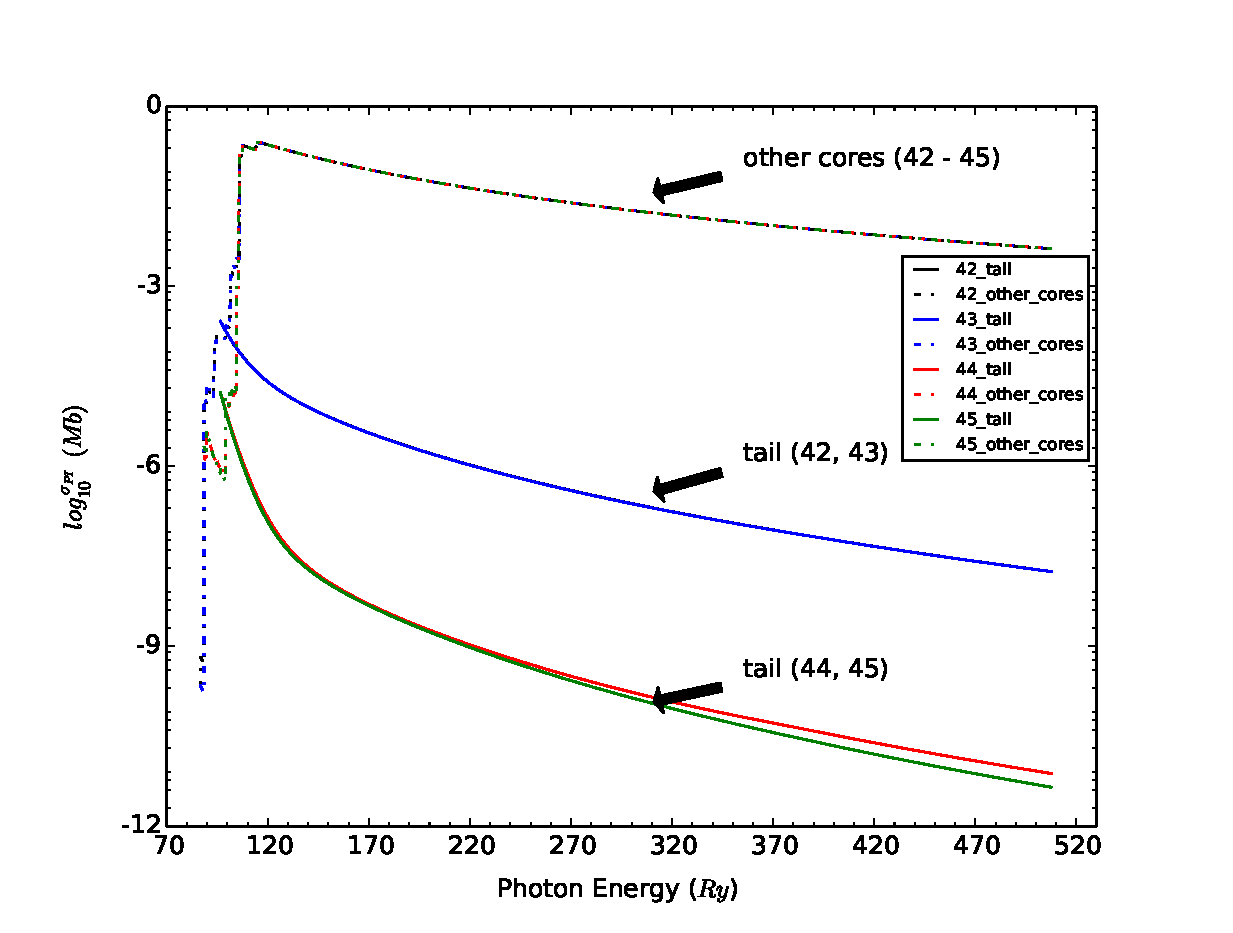
\includegraphics[width=.9\textwidth]{figures/fe18_mismatch_not_matter_tail_other.eps}
	\caption{\ion{Fe}{xviii}: The tail and the contribution from other core configurations of levels 42 - 45 as shown in table \ref{table_7_1_44} for both BPRM and RDW. }
	\label{fig_7_1_44_not_matter_tail_other}
\end{figure}

\subsubsection{Other Bound Levels}
In RDW, we consider all the bound state levels with $n\leq10$, so we collect all such levels that are not included in BPRM calculation, and calculate the photionization cross section due to all core configurations, i.e. the core configurations included in the BPRM calculation and the other ones displayed in section \ref{section_other_targets}, with different-n-complex configuration interaction. For \ion{Fe}{xvii}, there are extra 123 bound levels, while for \ion{Fe}{xviii} there are extra 428 bound levels, so it ends up with 587 bound levels in total for \ion{Fe}{xvii} and 1591 for \ion{Fe}{xviii}. To do a sanity check on the data, we show the photoionization cross section of two levels for each iron ion (see figure \ref{figure_other_levels}) and their energies are listed in table \ref{table_other_levels}. Since there is a big energy gap between $n=2$ and $n=3$ core configurations, the photoionization cross section should decrease smoothly without edges rising up predominantly just as in many figures shown in previous sections, and in figure \ref{figure_other_levels} we can observe such feature for all four levels. In the $n=3$ and $n=4$ core configurations energy region, the transitions are very likely dominated by the different-n-complex configuration interaction, creating many edges followed by a very fast descreasing tail, which is seen in figure \ref{figure_other_levels}. But if the bound level has configuration with the outer electron in $M-,~N-$shell, there will be a big jump in the photoionization cross section. For example, in each top panel of figures \ref{fe17_bprm_fac}, \ref{fe18_bprm_fac} and \ref{figure_fe17_bound_mix}, there is a big jump in the background of photoionization cross section, and RDW does an excellent job in reproducing it. As shown in chapter \ref{chap_pec_l_edge} these jumps are from the  PEC-L-Edge transitions (see table \ref{table_n3_n4_jumps}). In the higher energy region around $100~Ry$, all of the four levels have big jumps due to transitions shown in table \ref{table_n5_n6_jumps}. 

%======== Table other bound levels
\begin{table}
	\centering
	\caption{Listed are four of the bound levels found in the topup calculation and their photoionization cross section is shown in figure \ref{figure_other_levels}. Note: the energy is $z$-scaled ($z=17$ for \ion{Fe}{xvii} and 18 for \ion{Fe}{xviii}), and in unit of $10^{-3} Ry$.}
	\begin{tabular} { | c | c |}
		\hline
		Level & Energy \\
		\hline
		$2s^2 2p^5 10k~(J=8)$ & -6.7798\\
		$2s 2p^65f ~(J=2)$ & -5.8754\\
		$2s 2p^5 6g~(J=11/2)$ & -1.5446\\
		$2s 2p^5 6p~(J=5/2)$ & -1.2772\\
		\hline	  								   
	\end{tabular}
	\label{table_other_levels}
\end{table}

%======= Figure other levels
\begin{figure}
	\centering
	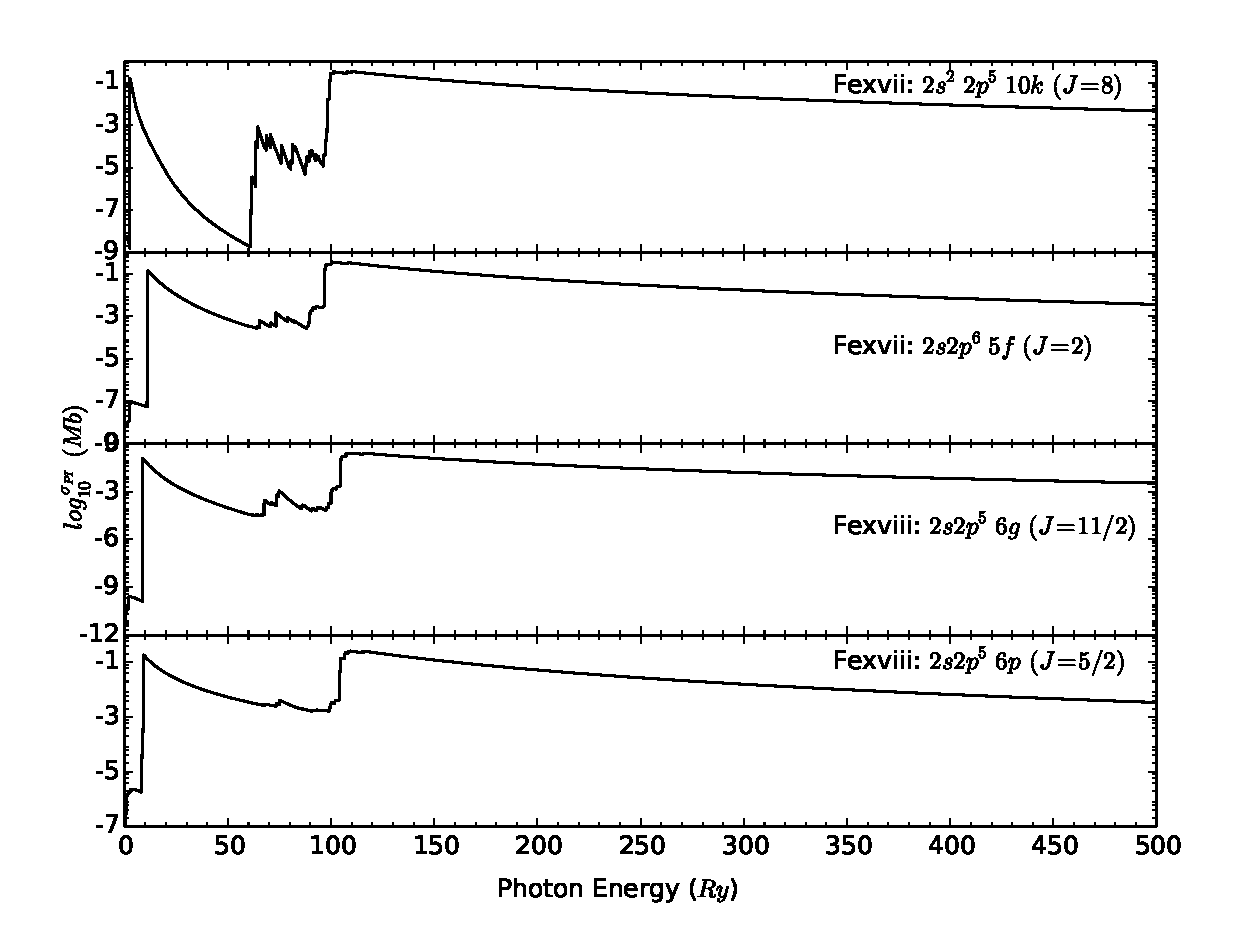
\includegraphics[width=.9\textwidth]{figures/other_levels.eps}
	\caption{Among the other bound levels, 2 of them for both \ion{Fe}{xvii} and \ion{Fe}{xviii} are shown. The configurations and $J$ values are provided. }
	\label{figure_other_levels}
\end{figure}

%======== Table n3 n4 jumps
\begin{table}
	\centering
	\caption{Listed are the main transitions that cause the jump of the background of photoionization cross section as shown in figures \ref{fe17_bprm_fac}, \ref{fe18_bprm_fac} and \ref{figure_fe17_bound_mix}.}
	\begin{tabular} { | c | c |}
		\hline
		Level & Final Configurations \\
		\hline
		$2s^2 2p^5 4d~(J=2)$ & $2s^2 2p^4 4d$, $2s 2p^5 4d$\\
		$2s^2 2p^4 4d~(J=5/2)$ & $2s^2 2p^3 4d$\\
		$2s^2 2p^5 3p~(J=0)$ & $2s^2 2p^4 3p$, $2s 2p^5 3p$\\
		\hline	  								   
	\end{tabular}
	\label{table_n3_n4_jumps}
\end{table}

%======== Table n5 n6 jumps
\begin{table}
	\centering
	\caption{Listed are the main transitions that cause the jump for levels with $n=5,~6,~10$, as shown in figure \ref{figure_other_levels}.}
	\begin{tabular} { | c | c |}
		\hline
		Level & Final Configurations \\
		\hline
		$2s^2 2p^5 10k~(J=8)$ & $2s^2 2p^4 10k$, $2s 2p^5 10k$\\
		$2s 2p^6 5f~(J=2)$ & $2s 2p^5 5f$, $2p^6 5f$\\
		$2s 2p^5 6g~(J=11/2)$ & $2s 2p^4 6g$, $2p^5 6g$\\
		$2s 2p^5 6p~(J=5/2)$ & $2s 2p^4 6p$, $2p^5 6p$\\
		\hline	  								   
	\end{tabular}
	\label{table_n5_n6_jumps}
\end{table}

\subsection{Bound - Bound} \label{section_bound_bound}
To top up the bound-bound oscillator strength, we divide it into two parts. One is from bound states to pure bound states. We calculate all the possible transitions, and only collect the ones that are not calculated in BPRM calculation. The other part is from bound states to quasi-bound states, i.e. doubly excited states. BPRM calculation  treats direct photionization and autoionization as a single quantum-mechanical process \citep{config_2003}, and in section \ref{section_bf}, direct photoionization is discussed, so to simulate the autoionization process, we calculate the oscillator strength from bound to doubly excited states, which is shown to reproduce the resonances very well \citep{ah_1997}. We consider the bound-quasi-bound transitions that excite an electron from $L$-shell to a higher one, forming a doubly excited configuration that can not be formed by combining a core configuration used in BPRM calculation with another electron.

%======= Table bound-bound fe17
\begin{table}
	\centering
	\caption{\ion{Fe}{xvii}: Bound-bound transitions included in the top up calculation. Note: $\ell$, $\ell'$ can be any subshell in each corresponding shell.}
	\label{table_fe17_bound_bound}
	\begin{tabular}{|c||c|c|}
		\hline
		Ion & Initial configurations & Final configurations \\
		\hline
		\multirow{19}{*}{\ion{Fe}{xvii}} & \multicolumn{2}{|c|}{Bound - Pure-Bound ($S+P=7$, $n \leq 10$)} \\
		\cline{2-3}
		& $2s^2 2p^6$ & $2s^S 2p^P n\ell$ ($n\geq3$) \\
		
		&$2s^S 2p^P 3\ell$ & $2s^S 2p^P n\ell$ ($n\geq3$) \\
		
		&$2s^S 2p^P 4\ell$ & $2s^S 2p^P n\ell$ ($n\geq4$) \\
		
		&$2s^S 2p^P 5\ell$ & $2s^S 2p^P n\ell$ ($n\geq5$) \\
		
		&$2s^S 2p^P 6\ell$ & $2s^S 2p^P n\ell$ ($n\geq6$) \\
		
		&$2s^S 2p^P 7\ell$ & $2s^S 2p^P n\ell$ ($n\geq7$) \\
		
		&$2s^S 2p^P 8\ell$ & $2s^S 2p^P n\ell$ ($n\geq8$) \\
		
		&$2s^S 2p^P 9\ell$ & $2s^S 2p^P n\ell$ ($n\geq9$) \\
		
		&$2s^S 2p^P 10\ell$ & $2s^S 2p^P n\ell$ ($n\geq10$) \\
		\cline{2-3}
		& \multicolumn{2}{|c|}{Bound - Quasi-Bound ($S+P=7$, $S'+P'=6$, $n \leq 7$)} \\
		\cline{2-3}
		& \multirow{3}{*} {$2s^S 2p^P 4\ell$} & $2p^6 4\ell n\ell'$ ($n\geq4$)\\
		& & $2s^2 2p^4 4f^2$, $2s^2 2p^4 4f n\ell$ ($n\geq5$) \\
		& & $2s 2p^5 4f^2$, $2s 2p^5 4f n\ell$ ($n\geq5$) \\
		\cline{3-3}
		& \multirow{2}{*} {$2s^S 2p^P 5\ell$} & $2p^6 4\ell 5\ell'$, $2s^2 2p^4 4f 5\ell$, $2s 2p^5 4f 5\ell$\\
		& & $2s^{S'} 2p^{P'} 5\ell n\ell'$ ($n\geq5$) \\
		\cline{3-3}	
		& \multirow{3}{*} {$2s^S 2p^P 6\ell$} & $2p^6 4\ell 6\ell'$, $2s^2 2p^4 4f 6\ell$, $2s 2p^5 4f 6\ell$\\
		& & $2s^{S'} 2p^{P'} 5\ell 6\ell'$\\
		& & $2s^{S'} 2p^{P'} 6\ell n\ell'$ ($n\geq6$)\\
		\cline{3-3}	
		& \multirow{2}{*} {$2s^S 2p^P 7\ell$} & $2p^6 4\ell 7\ell'$, $2s^2 2p^4 4f 7\ell$, $2s 2p^5 4f 7\ell$\\
		& & $2s^{S'} 2p^{P'} n\ell 7\ell'$ ($n\geq5$)\\ 							
		\hline
	\end{tabular}
\end{table}

%======= Table bound-bound fe18
\begin{table}
	\centering
	\caption{\ion{Fe}{xviii}: Bound-bound transitions included in the top up calculation. Note: $\ell$, $\ell'$ can be any subshell in each corresponding shell.}
	\label{table_fe18_bound_bound}
	\begin{tabular}{|c||c|c|}
		\hline
		Ion & Initial configurations & Final configurations \\
		\hline
		\multirow{19}{*}{\ion{Fe}{xviii}} & \multicolumn{2}{|c|}{Bound - Pure-Bound ($S+P=6$, $n \leq 10$)} \\
		\cline{2-3}
		& $2s^S 2p^P 2\ell$ & $2s^S 2p^P n\ell$ ($n\geq2$) \\
		
		&$2s^S 2p^P 3\ell$ & $2s^S 2p^P n\ell$ ($n\geq3$) \\
		
		&$2s^S 2p^P 4\ell$ & $2s^S 2p^P n\ell$ ($n\geq4$) \\
		
		&$2s^S 2p^P 5\ell$ & $2s^S 2p^P n\ell$ ($n\geq5$) \\
		
		&$2s^S 2p^P 6\ell$ & $2s^S 2p^P n\ell$ ($n\geq6$) \\
		
		&$2s^S 2p^P 7\ell$ & $2s^S 2p^P n\ell$ ($n\geq7$) \\
		
		&$2s^S 2p^P 8\ell$ & $2s^S 2p^P n\ell$ ($n\geq8$) \\
		
		&$2s^S 2p^P 9\ell$ & $2s^S 2p^P n\ell$ ($n\geq9$) \\
		
		&$2s^S 2p^P 10\ell$ & $2s^S 2p^P n\ell$ ($n\geq10$) \\
		\cline{2-3}
		& \multicolumn{2}{|c|}{Bound - Quasi-Bound ($S+P=6$, $S'+P' = 5$, $n \leq 7$)} \\
		\cline{2-3}
		& $2s^S 2p^P 3\ell$ & $2p^5 3\ell n\ell'$ ($n\geq 3$) \\
		\cline{3-3}
		& \multirow{3}{*} {$2s^S 2p^P 4\ell$} & $2s 2p^4 4\ell n\ell'$ ($n\geq4$)\\
		& & $2p^5 4\ell n\ell'$ ($n\geq3$) \\
		& & $2s^2 2p^3 4f^2$, $2s^2 2p^3 4f n\ell$ ($n\geq5$) \\
		\cline{3-3}
		& \multirow{4}{*} {$2s^S 2p^P 5\ell$} & $2s^2 2p^3 4f 5\ell$\\
		& & $2p^5 n\ell 5\ell' ($n = 3, 4$)$ \\
		& & $2s 2p^4 4\ell 5\ell'$ \\
		& & $2s^{S'} 2p^{P'} 5\ell n\ell'$  ($n \geq 5$)\\
		\cline{3-3}	
		& \multirow{4}{*} {$2s^S 2p^P 6\ell$} & $2s^2 2p^3 4f 6\ell$\\
		& & $2p^5 n\ell 6\ell' ($n = 3, 4$)$ \\
		& & $2s 2p^4 4\ell 6\ell'$ \\
		& & $2s^{S'} 2p^{P'} n\ell 6\ell'$  ($n \geq 5$)\\
		\cline{3-3}	
		& \multirow{4}{*} {$2s^S 2p^P 7\ell$} & $2s^2 2p^3 4f 7\ell$\\
		& & $2p^5 n\ell 7\ell' ($n = 3, 4$)$ \\
		& & $2s 2p^4 4\ell 7\ell'$ \\
		& & $2s^{S'} 2p^{P'} n\ell 7\ell'$  ($n \geq 5$)\\
		\hline
	\end{tabular}
\end{table}

\subsubsection{Bound - Pure-Bound}
In RDW calculation, we consider the bound configurations with principle quantum number up to 10 of the outer electron, and in BPRM calculation, some bound levels are missed out due to large scanning step and the upper scanning limit of the effective quantum number, thus in the bound to pure-bound transitions, we first calculate all the transitions possible between the bound configurations, which can only be formed by $n=2$ core configurations coupled with an outer electron. See the upper parts of tables \ref{table_fe17_bound_bound} and \ref{table_fe18_bound_bound} for \ion{Fe}{xvii} and \ion{Fe}{xviii}, respectively. Since we have obtained the level correspondence in BPRM and RDW through matching process as described in section \ref{section_matching}, we are readily to exclude the transitions between those levels, and keep the remaining bound to pure-bound transitions. There are some transitions between bound levels found in BPRM to quasi-bound levels which are formed by $n=2$ core configurations coupled with an outer electron, and these transitions are treated naturally as resonances in BPRM calculation, so in section \ref{section_bound_quasi_bound}, we do not include those transitions.  And we do not consider transitions between quasi-bound to quasi-bound levels, as quasi-bound means the levels have energy larger than the ground state of the core configurations, so they are essentially ionized and these transitions are unphysical in opacity calculation.

\subsubsection{Bound - Quasi-Bound}
\label{section_bound_quasi_bound}
Like the other parts of the top up calculation, the bound configurations only consider the same-n-complex configuration interaction. But with different-n-complex configuration interaction, there can be more transitions, e.g. from bound configurations $2s^2 2p^5 3\ell$ to quasi-bound configurations $2s^2 2p^4 4\ell 5\ell'$, though at the cost of losing bound level correspondence obtained in level-matching step as the energy is very likely to change, and to collect the energy information needed by the opacity calculation, the quasi-bound levels are readily available but the bound levels very likely have different energy from those that have already been collected in the bound to pure-bound transitions, and in this case maybe we can just neglect those changed energies, and use the previous one, so only quasi-bound level energy should be collected. Since the current data does not include such transitions, it might be another thing one can consider to improve on later, but it is very likely it will have negligible contribution to opacity. In the bound to quasi-bound top up calculation one can consider the transitions to the quasi-bound configurations with principle quantum number as high as interested, and in the current calculation we go up to 7, since the higher n introduces hundreds of thousands of quasi-bound levels, and it is very likely they are negligible compared with the big jump in photoionization cross section. In the following, I will give a detailed clarification on these transitions listed in tables \ref{table_fe17_bound_bound} and \ref{table_fe18_bound_bound}. 

In \ion{Fe}{xvii} 218 CCBPRM calculation, it includes complete $n=2$ core configurations, i.e. $2s^S 2p^P$, which can form possible quasi-bound configuratoins $2s^S 2p^P n\ell$. It also includes complete $n=3$ core configurations, i.e. $2s^{S'} 2p^{P'} 3\ell$ where $S'+P' = 6$, which can form possible quasi-bound configurations $2s^{S'} 2p^{P'} 3\ell n\ell'$ where $3 \leq n \leq 7$. And it includes part of the $n=4$ core configurations, i.e.  $2s^{S'} 2p^{P'} 4\ell$ where $S' = 1-2, ~\ell = 0-2$, which can form quasi-bound configurations $2s^{S'} 2p^{P'} 4\ell 4\ell'$, $2s^{S'} 2p^{P'} 4\ell n\ell'$ where $5 \leq n \leq 7$. Thus the bound levels in configurations $2s^2 2p^6$ and $2s^S 2p^P 3\ell$ are treated completely. For bound configurations $2s^S 2p^P 4\ell$, the resonances can be formed by transitions to possible quasi-bound configurations are $2s^S 2p^P n\ell$, $2s^{S'} 2p^{P'} 3\ell 4\ell'$, $2s^{S'} 2p^{P'} 4\ell 4\ell'$, $2s^{S'} 2p^{P'} 4\ell 5\ell'$, $2s^{S'} 2p^{P'} 4\ell 6\ell'$ and $2s^{S'} 2p^{P'} 4\ell 7\ell'$, of which the first two have already been included completely in BPRM and part of the rest are also included, leaving out $2p^6 4\ell n\ell'~(4 \leq n \leq 7)$, $2s^2 2p^4 4f^2$, $2s 2p^5 4f^2$, $2s^2 2p^4 4f n\ell$ and  $2s 2p^5 4f n\ell~(5 \leq n \leq 7)$ unconsidered. So in the top up calculation, we consider the transitions from  $2s^S 2p^P 4\ell$ to the quasi-bound configurations that are missed out. For the bound levels in configurations  $2s^S 2p^P 5\ell$, the possible quasi-bound configurations are  $2s^S 2p^P n\ell$,  $2s^{S'} 2p^{P'} 3\ell 5\ell'$, $2s^{S'} 2p^{P'} 4\ell 5\ell'$,  $2s^{S'} 2p^{P'} 5\ell n\ell'$ ($5 \leq n \leq 7$), so the missing configurations in BPRM are $2p^6 4\ell 5\ell'$, $2s^2 2p^4 4f 5\ell$, $2s 2p^5 4f 5\ell$, $2s^{S'} 2p^{P'} 5\ell n\ell'$ ($5 \leq n \leq 7$). As for bound levels in $2s^S 2p^P 6\ell$ and $2s^S 2p^P 7\ell$, it is very similar to $2s^S 2p^P 5\ell$, and the missing quasi-bound configurations are listed as shown in table \ref{table_fe17_bound_bound}.

In \ion{Fe}{xviii} 276 CCBPRM calculation, it includes complete $n=2$ core configurations, i.e. $2s^S  2p^P$, so it can form possible quasi-bound configurations $2s^S  2p^P n\ell$. It includes part of the $n=3$ core configurations, i.e. $2s^2 2p^3 3\ell$ and $2s 2p^4 3\ell$, and they can form possible quasi-bound configurations $2s^2 2p^3 3\ell n\ell'$ and $2s 2p^4 3\ell n\ell'$ ($3 \leq n \leq 6$). It also includes part of the $n=4$ core configurations, i.e. $2s^2 2p^3 4\ell$ ($\ell \leq 2$), and they can form quasi-bound configurations $2s^2 2p^3 4\ell n\ell'$ ($4 \leq n \leq 7$). So like \ion{Fe}{xvii}, bound levels in $2s^S 2p^P 2\ell$ are treated completely. For levels in bound configurations $2s^S 2p^P 3\ell$, the resonances can be due to transitions to quasi-bound configurations $2s^S 2p^P n\ell$ and  $2s^{S'} 2p^{P'} 3\ell n\ell'$ ($3 \leq n \leq 7$), so the missing quasi-bound configurations are $2p^5 3\ell n\ell'$ ($3 \leq n \leq 7$). For the bound levels in configuratoins $2s^S 2p^P 4\ell$, the possible quasi-bound configurations formed can be $2s^S 2p^P n\ell$, $2s^{S'} 2p^{P'} 3\ell 4\ell'$ and $2s^{S'} 2p^{P'} 4\ell n\ell'$ ($4 \leq n \leq 7$), so the missing configurations are $2p^5 3\ell 4\ell'$,  $2p^5 4\ell n\ell'$ ($4 \leq n \leq 7$), $2s 2p^4 4\ell n\ell'$ ($4 \leq n \leq 7$), $2s^2 2p^3 4f^2$ and $2s^2 2p^3 4f n\ell$ ($n = 5, ~6,~7$).  For the bound levels in configuratoins $2s^S 2p^P 5\ell$, the possible quasi-bound configurations formed can be $2s^S 2p^P n\ell$, $2s^{S'} 2p^{P'} 3\ell 5\ell'$, $2s^{S'} 2p^{P'} 4\ell 5\ell'$ and  $2s^{S'} 2p^{P'} 5\ell n\ell'$~($5 \leq n \leq 7$), so the missing configurations are $2p^5 3\ell 5\ell'$, $2s^2 2p^3 4f 5\ell$, $2s 2p^4 4\ell 5\ell'$, $2p^5 4\ell 5\ell'$ and $2s^{S'} 2p^{P'} 5\ell n\ell'$~($5 \leq n \leq 7$). For bound levels in $2s^S 2p^P 6\ell$ and  $2s^S 2p^P 7\ell$, it is very similar to $2s^S 2p^P 5\ell$, and the missing quasi-bound configurations are listed as shown in table \ref{table_fe18_bound_bound}.

\section{Conclusion}
Relativistic distorted wave calculation is performed for \ion{Fe}{xvii} and \ion{Fe}{xviii} to top-up the 218 and 276 CCBPRM calculation, respectively. Bound state levels are matched between BPRM and RDW calculation by comparing quantumn numbers $J$, $\pi$, energy, and photoionization cross section. With such level correspondance, the photoionization cross section of BPRM calculation in the higher energy region is extended using RDW data, and contribution from other core configurations up to $n=10$ is added. Other bound state levels are also included with photoionization cross section due to all the core configurations up to $n=10$. Including core configurations up to $n=10$ is crucial in that it ensures the PEC-L-Edge transitions for each bound state level, thus the jump showing up at around $100~Ry$ ensures the convergence of the photoionization cross section. Oscillator strength is also topped up, with contribution from bound-pure-bound transitions and bound-quasi-bound transitions with outer electron up to $n=7$. 
The effects of configuration interaction on photoionization cross section are discussed, including same-n-complex and different-n-complex, showing its significant role in reproducing the background of BPRM using RDW. Different-n-complex configuration interaction is important in the region before the PEC-L-Edge transitions kick in, and in some levels shown in figure \ref{figure_other_levels}, it changes the background dramatically in a few tens of Rydbergs. 